\documentclass[a4paper,12pt]{article}
\usepackage{standalone}
\usepackage[a4paper, top=0.8in, bottom=0.7in, left=0.8in, right=0.8in]{geometry}
\usepackage{amsmath}
\usepackage{hyperref}
\usepackage{amsfonts}
\usepackage{latexsym}
\usepackage{graphicx}
\usepackage{fancyhdr}
\usepackage{enumitem}
\usepackage{setspace}
\usepackage{tcolorbox}
\usepackage{tikz}
\usepackage{multicol}
\usepackage{xcolor}
\usepackage[defaultfam,tabular,lining]{montserrat} % Font settings for Montserrat

\usepackage{xcolor}  % To use colors
\hypersetup{
    colorlinks=true,   % Activate colored links
    linkcolor=blue,    % Link color for internal links
    urlcolor=blue,     % Link color for URLs
    filecolor=blue,    % Link color for file links
    menucolor=blue,    % Link color for menus
}



\sloppy

\title{}
\date{}
\hyphenpenalty=10000
\exhyphenpenalty=10000

\setlength{\parindent}{0pt}
\pagestyle{fancy}

\setlength{\headheight}{27.11148pt}
\addtolength{\topmargin}{-15.11148pt}

\fancyhf{}
\fancyhead[L]{\textbf{Curriculum G TWB}}
\fancyhead[R]{
\includegraphics[width=0.8cm]{Round Logo.png}} % Placeholder for logo
\fancyfoot[C]{\footnotesize © Study Smart Tutors}
\fancyfoot[R]{\thepage}  % Page number in bottom right corner
\fancyfoot[L]{\hyperlink{toc}{Back to Contents}} % Clickable link in bottom left to TOC

\sloppy

% Define a new command for the level letter
\newcommand{\levelLetter}{G}  % Change this letter to update throughout the document

% Define red and blue text for solutions and notes
\newcommand{\solution}[1]{\textcolor{red}{#1}}
\newcommand{\note}[1]{\textcolor{blue}{\textbf{Instructor Note: #1}}}

%%%%%%%%%%%%%%%%%%%%%%%%%%%%%%%%%%%%%

\begin{document}

% Title Page (Instructor Version)
\documentclass[12pt]{article}
\usepackage[a4paper, top=0.8in, bottom=0.7in, left=0.8in, right=0.8in]{geometry}
\usepackage{amsmath}
\usepackage{amsfonts}
\usepackage{latexsym}
\usepackage{graphicx}
\usepackage{tikz}
\usepackage{fancyhdr}
\usepackage{tcolorbox}
\usepackage{multicol}
\usepackage{tgadventor}
\renewcommand{\familydefault}{\sfdefault}
\usepackage{enumitem}
\usepackage{setspace}
\setlength{\parindent}{0pt}
\pagestyle{fancy}
\usepackage{needspace}


% Define a new command for the level letter
\newcommand{\levelLetter}{G}  % Change this letter to update throughout the document

%%%%%%%%%%%%%%%%%%%%%%%%%%%%%%%%%%%%%

\setlength{\headheight}{27.11148pt}
\addtolength{\topmargin}{-15.11148pt}

\fancyhf{}
%\fancyhead[L]{\textbf{5.NBT.A.1: Understand the Place Value System}}
\fancyhead[R]{
\includegraphics[width=0.8cm]{Round Logo.png}}
\fancyfoot[C]{\footnotesize © Study Smart Tutors}






\title{}
\date{}
\hyphenpenalty=10000
\exhyphenpenalty=10000

\begin{document}


%%%%%%%%%%%%%%%%%%%%%%%%%%%%%%%%%%%%%%%%%%%%%%%%%%%%%%%%%%%%%%%%%%%%


% INSTRUCTOR COVER PAGE BEGIN
% Skip header and footer on the first page
\thispagestyle{empty}

% Vertical centering
\vspace*{\fill}

\vspace*{3cm}

\begin{center}

    % Logo
    
\includegraphics[width=0.6\textwidth]{SST_Color_Logo.png} % Replace 'logo.png' with the path to your logo file
    
    \vspace{2cm} % Space between logo and title
    
    % Cycle Name

    
    % Assessment Title
    \Huge \textbf{Mathematics  Tutoring}\\
    [0.3cm]
     \vspace{1cm}
    \LARGE \textit{Curriculum \levelLetter}\\[1cm] 
   

    \Huge \textbf{INSTRUCTOR VERSION}
    
   
    
    \vfill % Push the footer to the bottom
    
\end{center}
\newpage
\thispagestyle{empty}
\vspace*{\fill}
\newpage

% INSTRUCTOR VERSION COVER PAGE COMPLETE




% *************************



\end{document}
 % Include the title page content here


\pagenumbering{gobble} 
\hypertarget{toc}{}  % Mark the TOC as a hyperlink target
% Table of Contents
\tableofcontents
\newpage



% Restart page numbering from 1 after TOC
\pagenumbering{arabic}
\pagestyle{fancy}  % Re-enable fancy headers/footers
% Guided Lesson and Problem Set for 6.NR.4.1, 6.NR.4.5
\newpage
\section{6.NR.4.1, 6.NR.4.5 Guided Lesson}
\documentclass[12pt]{article}
\usepackage[a4paper, top=0.8in, bottom=0.7in, left=0.8in, right=0.8in]{geometry}
\usepackage{amsmath}
\usepackage{amsfonts}
\usepackage{latexsym}
\usepackage{graphicx}
\usepackage{fancyhdr}
\usepackage{tcolorbox}
\usepackage{enumitem}
\usepackage{setspace}
\usepackage{xcolor} % For red and blue text
\usepackage[defaultfam,tabular,lining]{montserrat} % Font settings for Montserrat

% General Comment: Template for creating problem sets in a structured format with headers, titles, and sections.
% This document uses Montserrat font and consistent styles for exercises, problems, and performance tasks.

% -------------------------------------------------------------------
% Directions for LaTeX Styling and Content
% 1. Include a header with standards and topic title: \fancyhead[L]{\textbf{<Standards>: <Topic Title>}}.
% 2. Section Breakdown:
%    - Learning Objective: Concise goal statement.
%    - Exercises: Procedural fluency tasks.
%    - Problems: Moderately complex scenarios.
%    - Performance Task: Real-world, multi-step tasks.
%    - Reflection: Prompt to reflect on strategies and learning.
% -------------------------------------------------------------------

\setlength{\parindent}{0pt}
\pagestyle{fancy}

\setlength{\headheight}{27.11148pt}
\addtolength{\topmargin}{-15.11148pt}

\fancyhf{}
%\fancyhead[L]{\textbf{6.RP.A.1, 6.RP.A.2: Understanding Ratios and Unit Rates}} % Updated Header with standards and topic title
\fancyhead[R]{
\includegraphics[width=0.8cm]{Round Logo.png}} % Placeholder for logo
\fancyfoot[C]{\footnotesize © Study Smart Tutors}

\sloppy

\title{}
\date{}
\hyphenpenalty=10000
\exhyphenpenalty=10000

\begin{document}

\subsection*{Problem Set: Understanding Ratios and Unit Rates}
\onehalfspacing

% Learning Objective Box
\begin{tcolorbox}[colframe=black!40, colback=gray!5, 
coltitle=black, colbacktitle=black!20, fonttitle=\bfseries\Large, 
title=Learning Objective, halign title=center, left=5pt, right=5pt, top=5pt, bottom=15pt]
\textbf{Objective:} Understand and apply ratios and unit rates to solve problems in real-world contexts.  
\textcolor{blue}{\textbf{Instructor Note:} Use this section to clearly state the goal of the lesson. Emphasize that students will not only calculate ratios and rates but also interpret them in real-world scenarios.}
\end{tcolorbox}

% Key Concepts and Vocabulary Box
\begin{tcolorbox}[colframe=black!60, colback=white, 
coltitle=black, colbacktitle=black!15, fonttitle=\bfseries\Large, 
title=Key Concepts and Vocabulary, halign title=center, left=10pt, right=10pt, top=10pt, bottom=15pt]
\textbf{Key Concepts:}
\begin{itemize}
    \item \textbf{Ratios:} A ratio compares two quantities. It can be written as \( a:b \), \( \frac{a}{b} \), or "a to b."
    \item \textbf{Unit Rates:} A unit rate is a ratio where the second quantity is 1. For example, 60 miles per hour means 60 miles in 1 hour.
    \item \textbf{Equivalent Ratios:} Ratios are equivalent if they represent the same relationship, such as \( 2:4 \) and \( 1:2 \).
\end{itemize}
\textcolor{blue}{\textbf{Instructor Note:} Highlight these concepts during the lesson introduction. Consider using visual aids such as ratio tables or diagrams to demonstrate equivalent ratios and unit rates.}
\end{tcolorbox}

% Examples Box
\begin{tcolorbox}[colframe=black!60, colback=white, 
coltitle=black, colbacktitle=black!15, fonttitle=\bfseries\Large, 
title=Examples, halign title=center, left=10pt, right=10pt, top=10pt, bottom=15pt]
\textbf{Example 1: Understanding Ratios}  
\begin{itemize}
    \item Problem: A fruit basket contains 12 apples and 8 oranges. Write the ratio of apples to oranges.  
    \item Solution: The ratio of apples to oranges is \( 12:8 \). Simplify by dividing both numbers by 4: \( \textcolor{red}{12:8 = 3:2} \).  
\end{itemize}

\textbf{Example 2: Finding Unit Rates}  
\begin{itemize}
    \item Problem: A car drives 180 miles in 3 hours. What is the unit rate in miles per hour?  
    \item Solution: Divide the total miles by the total hours:  
    \[ \textcolor{red}{180 \div 3 = 60} \]  
    The unit rate is \( \textcolor{red}{60 \text{ miles per hour}} \).  
\end{itemize}
\textcolor{blue}{\textbf{Instructor Note:} Walk through each example step-by-step on the board. For Example 1, ask students to think of other real-world comparisons, such as students to teachers in a classroom. For Example 2, relate unit rates to speeds students are familiar with, such as walking or cycling speeds.}
\end{tcolorbox}

% Guided Practice Box
\begin{tcolorbox}[colframe=black!60, colback=white, 
coltitle=black, colbacktitle=black!15, fonttitle=\bfseries\Large, 
title=Guided Practice, halign title=center, left=10pt, right=10pt, top=10pt, bottom=15pt]
\textbf{Solve the following problems with teacher support:}
\begin{enumerate}[itemsep=3em]
    \item Write the ratio of blue marbles to green marbles if there are 9 blue marbles and 6 green marbles. Simplify the ratio.  
    \textcolor{red}{Solution: The ratio is \( 9:6 \). Simplify by dividing both numbers by 3: \( 9:6 = 3:2 \)}.  

    \item A bike covers 45 miles in 3 hours. Find the speed in miles per hour.  
    \textcolor{red}{Solution: Divide \( 45 \) by \( 3 \): \( 45 \div 3 = 15 \). The speed is \( 15 \text{ miles per hour} \)}.  
\end{enumerate}
\textcolor{blue}{\textbf{Instructor Note:} Encourage students to work collaboratively and explain their reasoning as they solve each problem. Offer guiding questions, such as, “What operation do we use to find the unit rate?”}
\end{tcolorbox}

% Independent Practice Box
\begin{tcolorbox}[colframe=black!60, colback=white, 
coltitle=black, colbacktitle=black!15, fonttitle=\bfseries\Large, 
title=Independent Practice, halign title=center, left=10pt, right=10pt, top=10pt, bottom=15pt]
\textbf{Solve the following problems independently:}
\begin{enumerate}[itemsep=3em]
    \item Write the ratio of 15 cats to 10 dogs. Simplify the ratio.  
    \textcolor{red}{Solution: The ratio is \( 15:10 \). Simplify by dividing both numbers by 5: \( 15:10 = 3:2 \)}.  

    \item A runner completes 24 miles in 6 hours. What is the runner's speed in miles per hour?  
    \textcolor{red}{Solution: Divide \( 24 \) by \( 6 \): \( 24 \div 6 = 4 \). The speed is \( 4 \text{ miles per hour} \)}.  

    \item A recipe calls for 2 cups of sugar for every 5 cups of flour. If you use 15 cups of flour, how much sugar is needed?  
    \textcolor{red}{Solution: Find the unit ratio: \( 2:5 \). Scale up: \( 2 \times 3 = 6 \). You need \( 6 \text{ cups of sugar} \)}.  
\end{enumerate}
\textcolor{blue}{\textbf{Instructor Note:} Monitor student progress and provide feedback as they work independently. Offer hints if students are stuck, such as suggesting they use multiplication tables to simplify ratios.}
\end{tcolorbox}

% Exit Ticket Box
\begin{tcolorbox}[colframe=black!60, colback=white, 
coltitle=black, colbacktitle=black!15, fonttitle=\bfseries\Large, 
title=Exit Ticket, halign title=center, left=10pt, right=10pt, top=10pt, bottom=15pt]
\textbf{Question:} A classroom has 12 boys and 16 girls. Write the ratio of boys to total students and simplify the ratio.  
\textcolor{red}{Solution: The total number of students is \( 12 + 16 = 28 \). The ratio is \( 12:28 \). Simplify by dividing both numbers by 4: \( 12:28 = 3:7 \)}. 

\textcolor{blue}{\textbf{Instructor Note:} Use the exit ticket to assess whether students can independently apply the day’s concepts. If needed, review simplifying ratios with the class before dismissing.}
\end{tcolorbox}

\end{document}


\newpage
\section{6.NR.4.1, 6.NR.4.5 Problem Set Answer Key}
\documentclass[12pt]{article}
\usepackage[a4paper, top=0.8in, bottom=0.7in, left=0.8in, right=0.8in]{geometry}
\usepackage{amsmath}
\usepackage{amsfonts}
\usepackage{latexsym}
\usepackage{graphicx}
\usepackage{fancyhdr}
\usepackage{tcolorbox}
\usepackage{enumitem}
\usepackage{setspace}
\usepackage[defaultfam,tabular,lining]{montserrat} % Font settings for Montserrat

\setlength{\parindent}{0pt}
\pagestyle{fancy}

\setlength{\headheight}{27.11148pt}
\addtolength{\topmargin}{-15.11148pt}

\fancyhf{}
%\fancyhead[L]{\textbf{6.RP.A.1, 6.RP.A.2: Understanding Ratios and Unit Rates - Answer Key}}
\fancyhead[R]{
\includegraphics[width=0.8cm]{Round Logo.png}}
\fancyfoot[C]{\footnotesize © Study Smart Tutors}

\sloppy

\title{}
\date{}
\hyphenpenalty=10000
\exhyphenpenalty=10000

\begin{document}

\subsection*{Problem Set: Understanding Ratios and Unit Rates - Answer Key}
\onehalfspacing

% Learning Objective Box
\begin{tcolorbox}[colframe=black!40, colback=gray!5, 
coltitle=black, colbacktitle=black!20, fonttitle=\bfseries\Large, 
title=Learning Objective, halign title=center, left=5pt, right=5pt, top=5pt, bottom=15pt]
\textbf{Objective:} Understand and apply ratios and unit rates to solve problems in real-world contexts.
\end{tcolorbox}

% Exercises Box
\begin{tcolorbox}[colframe=black!60, colback=white, 
coltitle=black, colbacktitle=black!15, fonttitle=\bfseries\Large, 
title=Exercises, halign title=center, left=10pt, right=10pt, top=10pt, bottom=60pt]
\begin{enumerate}[itemsep=1.35em]
    \item Write the ratio of pencils to pens if there are 8 pencils and 12 pens.\\
    \textcolor{red}{\textbf{Solution:} The ratio is \(8:12\), which simplifies to \(2:3\).}

    \item Simplify the ratio \(24:36\).\\
    \textcolor{red}{\textbf{Solution:} Divide both terms by the greatest common factor (\(12\)): \(24 \div 12 : 36 \div 12 = 2:3\).}

    \item Write \(3:5\) as a fraction, decimal, and percentage.\\
    \textcolor{red}{\textbf{Solution:} Fraction: \(\frac{3}{5}\); Decimal: \(0.6\); Percentage: \(0.6 \times 100 = 60\%\).}

    \item Find the unit rate: If 200 miles are driven in 4 hours, what is the speed in miles per hour?\\
    \textcolor{red}{\textbf{Solution:} Unit rate: \(200 \div 4 = 50\). The speed is \(50\) miles per hour.}

    \item A fruit basket contains 15 apples and 10 bananas. Write the ratio of apples to bananas in simplest form.\\
    \textcolor{red}{\textbf{Solution:} The ratio is \(15:10\), which simplifies to \(3:2\).}

    \item A car travels 150 miles in 3 hours. Write the ratio of miles to hours and calculate the unit rate.\\
    \textcolor{red}{\textbf{Solution:} Ratio: \(150:3\); Unit rate: \(150 \div 3 = 50\). The car travels \(50\) miles per hour.}

    \item Complete the table of equivalent ratios:
    \[
    \begin{array}{|c|c|c|c|}
    \hline
    4 & 8 & 12 & \_\_\_\_ \\
    \hline
    5 & 10 & 15 & \_\_\_\_ \\
    \hline
    \end{array}
    \]
    \textcolor{red}{\textbf{Solution:} The missing values are \(16\) and \(20\), since the equivalent ratio is consistent: \(4:5 = 8:10 = 12:15 = 16:20\).}

    \item Provide an example from everyday life that illustrates the ratio \( 7:3 \), and explain its significance.\\
    \textcolor{red}{\textbf{Solution:} Example: A recipe calls for \(7\) cups of water for every \(3\) cups of rice. This means for every 3 cups of rice used, 7 cups of water must be added to maintain the correct consistency.}
\end{enumerate}
\end{tcolorbox}

% Problems Box
\begin{tcolorbox}[colframe=black!60, colback=white, 
coltitle=black, colbacktitle=black!15, fonttitle=\bfseries\Large, 
title=Problems, halign title=center, left=10pt, right=10pt, top=10pt, bottom=80pt]
\begin{enumerate}[start=9, itemsep=2em]
    \item Determine whether the ratio \(9:12\) is equivalent to \(3:4\). Justify your answer.\\
    \textcolor{red}{\textbf{Solution:} Simplify \(9:12\): \(9 \div 3 : 12 \div 3 = 3:4\). Yes, they are equivalent.}

    \item Given the table of ratios below, identify which ratios are equivalent to \(2:3\):  
    \[
    \begin{array}{|c|c|c|c|}
    \hline
    4:6 & 6:8 & 8:12 & 10:15 \\
    \hline
    \end{array}
    \]
    \textcolor{red}{\textbf{Solution:} Equivalent ratios are \(4:6\), \(8:12\), and \(10:15\). These simplify to \(2:3\). \(6:8\) simplifies to \(3:4\), so it is not equivalent.}

    \item If the ratio of red to blue marbles in a bag is \(3:2\) and there are 25 marbles in total, how many of each color are there?\\
    \textcolor{red}{\textbf{Solution:} The total parts are \(3 + 2 = 5\). Each part represents \(25 \div 5 = 5\). Red: \(3 \times 5 = 15\); Blue: \(2 \times 5 = 10\).}

    \item A recipe calls for 2 cups of sugar for every 3 cups of flour. If you use 12 cups of flour, how much sugar will you need?\\
    \textcolor{red}{\textbf{Solution:} Set up a ratio: \(2:3 = x:12\). Solve for \(x\): \(x = (2 \times 12) \div 3 = 8\). You will need \(8\) cups of sugar.}

    \item A classroom has 18 boys and 12 girls. What is the ratio of boys to total students?\\
    \textcolor{red}{\textbf{Solution:} Total students: \(18 + 12 = 30\). Ratio of boys to total students: \(18:30\), which simplifies to \(3:5\).}

    \item A store sells 5 oranges for \$2. What is the cost per orange?\\
    \textcolor{red}{\textbf{Solution:} Unit rate: \(2 \div 5 = 0.4\). The cost per orange is \$0.40.}
\end{enumerate}
\end{tcolorbox}

% Performance Task Box
\begin{tcolorbox}[colframe=black!60, colback=white, 
coltitle=black, colbacktitle=black!15, fonttitle=\bfseries\Large, 
title=Performance Task: Designing a Garden, halign title=center, left=10pt, right=10pt, top=10pt, bottom=80pt]
You are designing a rectangular garden. Here’s what you know:
\begin{itemize}
    \item The ratio of flower beds to vegetable beds is \(3:2\).
    \item There are 15 flower beds in the garden.
    \item Each vegetable bed requires 1.5 square meters of soil.
\end{itemize}

\textbf{Task:}
\begin{enumerate}[itemsep=4em]
    \item Calculate the number of vegetable beds in the garden.\\
    \textcolor{red}{\textbf{Solution:} Using the ratio \(3:2\), the total parts are \(3 + 2 = 5\). Each part represents \(15 \div 3 = 5\). Vegetable beds: \(2 \times 5 = 10\).}

    \item Determine the total area of soil required for the vegetable beds.\\
    \textcolor{red}{\textbf{Solution:} Each vegetable bed requires \(1.5\) square meters. Total: \(10 \times 1.5 = 15\) square meters.}

    \item Write the ratio of total flower beds to total beds in the garden.\\
    \textcolor{red}{\textbf{Solution:} Total beds: \(15 + 10 = 25\). Ratio: \(15:25\), which simplifies to \(3:5\).}

    \item Explain how understanding ratios helps in designing the garden layout.\\
    \textcolor{red}{\textbf{Solution:} Ratios help allocate space proportionally between flower and vegetable beds, ensuring proper use of the area.}
\end{enumerate}
\end{tcolorbox}

% Reflection Box
\begin{tcolorbox}[colframe=black!60, colback=white, 
coltitle=black, colbacktitle=black!15, fonttitle=\bfseries\Large, 
title=Reflection, halign title=center, left=10pt, right=10pt, top=10pt, bottom=100pt]
What strategies did you use to solve ratio problems? Share any patterns or connections you noticed during the exercises and tasks.
\end{tcolorbox}

\end{document}


% Guided Lesson and Problem Set for 6.NR.4.3
\newpage
\section{6.NR.4.3 Guided Lesson}
\documentclass[12pt]{article}
\usepackage[a4paper, top=0.8in, bottom=0.7in, left=0.8in, right=0.8in]{geometry}
\usepackage{amsmath}
\usepackage{amsfonts}
\usepackage{latexsym}
\usepackage{graphicx}
\usepackage{fancyhdr}
\usepackage{tcolorbox}
\usepackage{enumitem}
\usepackage{setspace}
\usepackage{xcolor}
\usepackage[defaultfam,tabular,lining]{montserrat} % Font settings for Montserrat

% General Comment: Template for creating problem sets in a structured format with headers, titles, and sections.
% This document uses Montserrat font and consistent styles for exercises, problems, and performance tasks.

% -------------------------------------------------------------------
% Directions for LaTeX Styling and Content
% 1. Include a header with standards and topic title: \fancyhead[L]{\textbf{<Standards>: <Topic Title>}}.
% 2. Section Breakdown:
%    - Learning Objective: Concise goal statement.
%    - Key Concepts and Vocabulary: Definitions and explanations.
%    - Examples: Worked-out problems.
%    - Guided Practice: Supported practice problems.
%    - Independent Practice: Problems for students to solve individually.
%    - Exit Ticket: Summative question to check understanding.
% -------------------------------------------------------------------

\setlength{\parindent}{0pt}
\pagestyle{fancy}

\setlength{\headheight}{27.11148pt}
\addtolength{\topmargin}{-15.11148pt}

\fancyhf{}
%\fancyhead[L]{\textbf{6.RP.A.3: Ratios, Proportions, and Problem Solving}}
\fancyhead[R]{
\includegraphics[width=0.8cm]{Round Logo.png}} % Placeholder for logo
\fancyfoot[C]{\footnotesize © Study Smart Tutors}

\sloppy

\title{}
\date{}
\hyphenpenalty=10000
\exhyphenpenalty=10000

\begin{document}

\subsection*{Guided Lesson: Ratios, Proportions, and Problem Solving}
\onehalfspacing

% Learning Objective Box
\begin{tcolorbox}[colframe=black!40, colback=gray!5, 
coltitle=black, colbacktitle=black!20, fonttitle=\bfseries\Large, 
title=Learning Objective, halign title=center, left=5pt, right=5pt, top=5pt, bottom=15pt]
\textbf{Objective:} Understand and solve real-world problems using ratio and rate reasoning with representations such as tables, tape diagrams, and double number lines.

\textcolor{blue}{\textbf{Instructor Note:} Emphasize that the goal is for students to connect ratios and rates to real-world scenarios. Provide visual aids such as ratio tables or double number lines for students who may benefit from visual representations.}
\end{tcolorbox}

% Key Concepts and Vocabulary Box
\begin{tcolorbox}[colframe=black!60, colback=white, 
coltitle=black, colbacktitle=black!15, fonttitle=\bfseries\Large, 
title=Key Concepts and Vocabulary, halign title=center, left=10pt, right=10pt, top=10pt, bottom=15pt]
\textbf{Key Concepts:}
\begin{itemize}
    \item A \textbf{ratio} is a comparison of two quantities, often written as \( a:b \), \( \frac{a}{b} \), or "a to b."
    \item A \textbf{rate} is a ratio that compares two quantities measured in different units, such as miles per hour or price per item.
    \item \textbf{Proportions} are equations that state two ratios are equivalent, such as \( \frac{a}{b} = \frac{c}{d} \).
    \item \textbf{Unit rate} is the value of one quantity for one unit of another, such as cost per item.
\end{itemize}

\textcolor{blue}{\textbf{Instructor Note:} Use examples from students' daily lives, such as comparing prices at a store or calculating speed during a trip, to help them relate to these concepts.}
\end{tcolorbox}

% Examples Box
\begin{tcolorbox}[colframe=black!60, colback=white, 
coltitle=black, colbacktitle=black!15, fonttitle=\bfseries\Large, 
title=Examples, halign title=center, left=10pt, right=10pt, top=10pt, bottom=15pt]
\textbf{Example 1: Finding Ratios}
\begin{itemize}
    \item Problem: Write the ratio of apples to oranges if there are 8 apples and 12 oranges.
    \item \textcolor{red}{Solution: Write the ratio as \( 8:12 \). Simplify by dividing both parts by their GCF, which is 4. \( 8 \div 4 : 12 \div 4 = 2:3 \). The simplified ratio is \( 2:3 \).}
\end{itemize}

\textbf{Example 2: Solving a Proportion}
\begin{itemize}
    \item Problem: Solve \( \frac{3}{4} = \frac{x}{12} \).
    \item \textcolor{red}{Solution: Use cross-multiplication: \( 3 \cdot 12 = 4 \cdot x \). This gives \( 36 = 4x \). Divide both sides by 4: \( x = \frac{36}{4} = 9 \). The solution is \( x = 9 \).}
\end{itemize}

\textcolor{blue}{\textbf{Instructor Note:} Highlight how cross-multiplication works and why it is a useful tool for solving proportions. Encourage students to double-check their work by substituting the solution back into the original proportion.}
\end{tcolorbox}

% Guided Practice Box
\begin{tcolorbox}[colframe=black!60, colback=white, 
coltitle=black, colbacktitle=black!15, fonttitle=\bfseries\Large, 
title=Guided Practice, halign title=center, left=10pt, right=10pt, top=10pt, bottom=15pt]
\textbf{Solve the following problems with teacher support:}
\begin{enumerate}[itemsep=3em]
    \item A recipe calls for \( 2 \) cups of sugar for every \( 3 \) cups of flour. How much sugar is needed for 12 cups of flour?\\
    \textcolor{red}{Solution: Set up a proportion: \( \frac{2}{3} = \frac{x}{12} \). Cross-multiply: \( 3x = 24 \). Solve for \( x \): \( x = 8 \). You need \( 8 \, \text{cups of sugar} \).}
    
    \item A car travels 120 miles in 2 hours. What is the unit rate in miles per hour?\\
    \textcolor{red}{Solution: Divide distance by time: \( 120 \div 2 = 60 \). The car travels \( 60 \, \text{miles per hour} \).}
\end{enumerate}

\textcolor{blue}{\textbf{Instructor Note:} Work through these problems collaboratively with students, emphasizing the steps to set up and solve proportions. Encourage students to explain their reasoning as they work.}
\end{tcolorbox}

% Independent Practice Box
\begin{tcolorbox}[colframe=black!60, colback=white, 
coltitle=black, colbacktitle=black!15, fonttitle=\bfseries\Large, 
title=Independent Practice, halign title=center, left=10pt, right=10pt, top=10pt, bottom=15pt]
\textbf{Solve the following problems independently:}
\begin{enumerate}[itemsep=3em]
    \item Simplify the ratio \( 24:36 \).\\
    \textcolor{red}{Solution: Divide both parts by their GCF (12): \( 24 \div 12 : 36 \div 12 = 2:3 \).}

    \item A map has a scale of \( 1 \, \text{inch} = 50 \, \text{miles} \). What is the actual distance for \( 3.5 \, \text{inches} \)?\\
    \textcolor{red}{Solution: Multiply: \( 3.5 \cdot 50 = 175 \, \text{miles} \).}

    \item Complete the table for a rate of \$15 per hour:
    \[
    \begin{array}{|c|c|c|c|}
    \hline
    \text{Hours} & 3 & 4 & 5 \\
    \hline
    \text{Earnings (\$)} & 45 & 60 & 75 \\
    \hline
    \end{array}
    \]
    \textcolor{red}{Solution: Multiply each hour by \$15.}
\end{enumerate}

\textcolor{blue}{\textbf{Instructor Note:} Encourage students to check their work and explain how they arrived at their answers. Offer guidance to students who struggle with setting up proportions or simplifying ratios.}
\end{tcolorbox}

% Exit Ticket Box
\begin{tcolorbox}[colframe=black!60, colback=white, 
coltitle=black, colbacktitle=black!15, fonttitle=\bfseries\Large, 
title=Exit Ticket, halign title=center, left=10pt, right=10pt, top=10pt, bottom=15pt]
\textbf{Answer the following question:}
\begin{itemize}
    \item A delivery truck travels 300 miles using 10 gallons of fuel. What is the unit rate in miles per gallon?\\
    \textcolor{red}{Solution: Divide \( 300 \div 10 = 30 \, \text{miles per gallon} \).}
\end{itemize}

\textcolor{blue}{\textbf{Instructor Note:} Use student responses to the exit ticket as a quick assessment of understanding. Follow up with reteaching as necessary.}
\end{tcolorbox}

\end{document}


\newpage
\section{6.NR.4.3 Problem Set Answer Key}
\documentclass[12pt]{article}
\usepackage[a4paper, top=0.8in, bottom=0.7in, left=0.8in, right=0.8in]{geometry}
\usepackage{amsmath}
\usepackage{amsfonts}
\usepackage{latexsym}
\usepackage{graphicx}
\usepackage{fancyhdr}
\usepackage{tcolorbox}
\usepackage{enumitem}
\usepackage{setspace}
\usepackage[defaultfam,tabular,lining]{montserrat} % Font settings for Montserrat

\setlength{\parindent}{0pt}
\pagestyle{fancy}

\setlength{\headheight}{27.11148pt}
\addtolength{\topmargin}{-15.11148pt}

\fancyhf{}
%\fancyhead[L]{\textbf{6.RP.A.3: Ratios, Proportions, and Problem Solving - Answer Key}}
\fancyhead[R]{
\includegraphics[width=0.8cm]{Round Logo.png}}
\fancyfoot[C]{\footnotesize © Study Smart Tutors}

\sloppy

\title{}
\date{}
\hyphenpenalty=10000
\exhyphenpenalty=10000

\begin{document}

\subsection*{Problem Set: Understanding Ratios and Proportions - Answer Key}
\onehalfspacing

% Learning Objective Box
\begin{tcolorbox}[colframe=black!40, colback=gray!5, 
coltitle=black, colbacktitle=black!20, fonttitle=\bfseries\Large, 
title=Learning Objective, halign title=center, left=5pt, right=5pt, top=5pt, bottom=15pt]
\textbf{Objective:} Understand and solve real-world problems using ratio and rate reasoning with representations such as tables, tape diagrams, and double number lines.
\end{tcolorbox}

% Exercises Box
\begin{tcolorbox}[colframe=black!60, colback=white, 
coltitle=black, colbacktitle=black!15, fonttitle=\bfseries\Large, 
title=Exercises, halign title=center, left=10pt, right=10pt, top=10pt, bottom=60pt]
\begin{enumerate}[itemsep=2em]
    \item Write the ratio of apples to oranges in a basket if there are 8 apples and 12 oranges.\\
    \textcolor{red}{\textbf{Solution:} The ratio is \( 8:12 \), which simplifies to \( 2:3 \) by dividing both terms by 4.}

    \item Simplify the ratio \( 24:36 \) to its simplest form.\\
    \textcolor{red}{\textbf{Solution:} \( 24 \div 12 : 36 \div 12 = 2:3 \), since 12 is the greatest common factor.}

    \item If a car travels 180 miles in 3 hours, what is the unit rate in miles per hour?\\
    \textcolor{red}{\textbf{Solution:} \( 180 \div 3 = 60 \). The unit rate is \( 60 \, \text{mph} \).}

    \item Solve: \( 6x = 54 \). Write your answer and verify it.\\
    \textcolor{red}{\textbf{Solution:} Divide both sides by 6: \( x = \frac{54}{6} = 9 \). Verification: \( 6 \times 9 = 54 \).}

    \item A bag of rice weighs \( 2.5 \) kilograms. How many grams is that? (Hint: \( 1 \, \text{kg} = 1000 \, \text{g} \)).\\
    \textcolor{red}{\textbf{Solution:} \( 2.5 \times 1000 = 2500 \, \text{grams} \).}

    \item Write a proportion for the statement: "Four pencils cost \$6, so eight pencils cost \$x."\\
    \textcolor{red}{\textbf{Solution:} Proportion: \( \frac{4}{6} = \frac{8}{x} \).}

    \item Find the missing value in the proportion: \( \frac{3}{4} = \frac{x}{12} \).\\
    \textcolor{red}{\textbf{Solution:} Cross-multiply: \( 3 \times 12 = 4x \). Solve: \( x = \frac{36}{4} = 9 \).}

    \item Convert \( 3:4 \) into a fraction and a decimal.\\
    \textcolor{red}{\textbf{Solution:} Fraction: \( \frac{3}{4} \); Decimal: \( 0.75 \).}
\end{enumerate}
\end{tcolorbox}

% Problems Box
\begin{tcolorbox}[colframe=black!60, colback=white, 
coltitle=black, colbacktitle=black!15, fonttitle=\bfseries\Large, 
title=Problems, halign title=center, left=10pt, right=10pt, top=10pt, bottom=60pt]
\begin{enumerate}[start=9, itemsep=2em]
    \item A recipe calls for \( 2 \) cups of flour for every \( 3 \) cups of sugar. How much flour is needed if 12 cups of sugar are used?\\
    \textcolor{red}{\textbf{Solution:} Ratio: \( 2:3 \). Set up the proportion: \( \frac{2}{3} = \frac{x}{12} \). Cross-multiply: \( 2 \times 12 = 3x \). Solve: \( x = 8 \). You need 8 cups of flour.}

    \item A map has a scale of \( 1 \, \text{inch} = 50 \, \text{miles} \). What is the actual distance represented by \( 3.5 \) inches on the map?\\
    \textcolor{red}{\textbf{Solution:} Multiply: \( 3.5 \times 50 = 175 \). The actual distance is \( 175 \, \text{miles} \).}

    \item Complete the table to represent the relationship between hours worked and earnings at a rate of \$15 per hour:
    \[
    \begin{array}{|c|c|c|c|}
    \hline
    \text{Hours} & 3 & 4 & 5 \\
    \hline
    \text{Earnings (\$)} & 45 & 60 & 75 \\
    \hline
    \end{array}
    \]
    \textcolor{red}{\textbf{Solution:} Multiply each hour value by 15: \( 3 \times 15 = 45 \), \( 4 \times 15 = 60 \), \( 5 \times 15 = 75 \).}

    \item A factory produces 240 widgets in \( 8 \) hours. At this rate, how many widgets can it produce in \( 12 \) hours?\\
    \textcolor{red}{\textbf{Solution:} Unit rate: \( 240 \div 8 = 30 \, \text{widgets/hour} \). Total for 12 hours: \( 30 \times 12 = 360 \, \text{widgets} \).}

    \item If \( \frac{7}{x} = \frac{28}{36} \), solve for \( x \).\\
    \textcolor{red}{\textbf{Solution:} Cross-multiply: \( 7 \times 36 = 28x \). Solve: \( x = \frac{252}{28} = 9 \).}

    \item Two buses leave a station. One travels at \( 45 \, \text{mph} \), and the other at \( 55 \, \text{mph} \). If they start at the same time, how far apart will they be after \( 2 \, \text{hours} \)?\\
    \textcolor{red}{\textbf{Solution:} Distance difference per hour: \( 55 - 45 = 10 \, \text{mph} \). After 2 hours: \( 10 \times 2 = 20 \, \text{miles} \).}
\end{enumerate}
\end{tcolorbox}

% Performance Task Box
\begin{tcolorbox}[colframe=black!60, colback=white, 
coltitle=black, colbacktitle=black!15, fonttitle=\bfseries\Large, 
title=Performance Task: Planning a Road Trip, halign title=center, left=10pt, right=10pt, top=10pt, bottom=80pt]
\textbf{Scenario:} You are planning a road trip with friends. The car consumes \( 1 \) gallon of fuel for every \( 25 \) miles, and the total distance of the trip is \( 300 \) miles.

\textbf{Task:}
\begin{enumerate}[itemsep=5em]
    \item Write a proportion to calculate the amount of fuel needed for the trip. Solve for the total gallons required.\\
    \textcolor{red}{\textbf{Solution:} Proportion: \( \frac{1}{25} = \frac{x}{300} \). Cross-multiply: \( 25x = 300 \). Solve: \( x = 12 \). You need 12 gallons of fuel.}

    \item If fuel costs \$4 per gallon, how much will the total cost of fuel be for the trip?\\
    \textcolor{red}{\textbf{Solution:} Total cost: \( 12 \times 4 = 48 \). The total fuel cost is \$48.}

    \item If the car’s tank holds \( 12 \) gallons, how many times will you need to refuel during the trip?\\
    \textcolor{red}{\textbf{Solution:} Since the tank holds exactly 12 gallons, you won’t need to refuel during the trip.}
\end{enumerate}
\end{tcolorbox}

% Reflection Box
\begin{tcolorbox}[colframe=black!60, colback=white, 
coltitle=black, colbacktitle=black!15, fonttitle=\bfseries\Large, 
title=Reflection, halign title=center, left=10pt, right=10pt, top=10pt, bottom=100pt]
Think about the problems you solved today. What was the most challenging part, and how did you work through it? Share one example of how you might use these skills in your daily life.
\end{tcolorbox}

\end{document}


% Guided Lesson and Problem Set for 6.NR.1.2
\newpage
\section{6.NR.1.2 Guided Lesson}
\documentclass[12pt]{article}
\usepackage[a4paper, top=0.8in, bottom=0.7in, left=0.8in, right=0.8in]{geometry}
\usepackage{amsmath}
\usepackage{amsfonts}
\usepackage{latexsym}
\usepackage{graphicx}
\usepackage{fancyhdr}
\usepackage{enumitem}
\usepackage{setspace}
\usepackage{tikz}
\usepackage{tcolorbox}
\usepackage{textcomp}
\usepackage[defaultfam,tabular,lining]{montserrat} % Font settings for Montserrat

\setlength{\parindent}{0pt}
\pagestyle{fancy}

\setlength{\headheight}{27.11148pt}
\addtolength{\topmargin}{-15.11148pt}

\fancyhf{}
%\fancyhead[L]{\textbf{6.NS.A.1: Dividing Fractions by Fractions}} % Header with standards and topic title
\fancyhead[R]{
\includegraphics[width=0.8cm]{Round Logo.png}} % Placeholder for logo
\fancyfoot[C]{\footnotesize © Study Smart Tutors}

\sloppy

\newcommand{\dsfrac}[2]{\dsfrac{#1}{#2}} % New command for display style fractions

\title{}
\date{}
\hyphenpenalty=10000
\exhyphenpenalty=10000

\begin{document}

\subsection*{Guided Lesson: Dividing Fractions by Fractions}
\onehalfspacing

% Learning Objective Box
\begin{tcolorbox}[colframe=black!40, colback=gray!5, 
coltitle=black, colbacktitle=black!20, fonttitle=\bfseries\Large, 
title=Learning Objective, halign title=center, left=5pt, right=5pt, top=5pt, bottom=15pt]
\textbf{Objective:} Interpret and compute quotients of fractions to solve real-world and mathematical problems involving division of fractions by fractions.
\textcolor{blue}{Instructor Note: Ensure students understand the goal is not just computation but also real-world interpretation. Emphasize the connection between dividing fractions and multiplication by reciprocals.}
\end{tcolorbox}

% Key Concepts and Vocabulary
\begin{tcolorbox}[colframe=black!60, colback=white, 
coltitle=black, colbacktitle=black!15, fonttitle=\bfseries\Large, 
title=Key Concepts and Vocabulary, halign title=center, left=10pt, right=10pt, top=10pt, bottom=15pt]
\textbf{Key Concepts:}
\begin{itemize}
    \item \textbf{Dividing Fractions:} To divide fractions, multiply the first fraction by the reciprocal of the second fraction.
    \item \textbf{Reciprocal:} The reciprocal of a fraction \( \frac{a}{b} \) is \( \frac{b}{a} \). For example, the reciprocal of \( \frac{2}{3} \) is \( \frac{3}{2} \).
    \item \textbf{Real-World Interpretation:} Division of fractions can represent how many groups of one fraction are in another, or the size of one group when a total is shared equally.
\end{itemize}
\textcolor{blue}{Instructor Note: Use visual models or manipulatives to demonstrate the concept of reciprocals and fraction division. This is particularly helpful for students struggling with abstract reasoning.}
\end{tcolorbox}

\vspace{1em}

% Examples Box
\begin{tcolorbox}[colframe=black!60, colback=white, 
coltitle=black, colbacktitle=black!15, fonttitle=\bfseries\Large, 
title=Examples, halign title=center, left=10pt, right=10pt, top=10pt, bottom=15pt]
\textbf{Example 1: Dividing Two Fractions}
\begin{itemize}
    \item Problem: Divide \( \frac{3}{4} \div \frac{1}{2} \).
    \item Solution:
    \textcolor{red}{Step 1: Rewrite the division as multiplication by the reciprocal of \( \frac{1}{2} \): 
    \[
    \frac{3}{4} \div \frac{1}{2} = \frac{3}{4} \times \frac{2}{1}.
    \]
    Step 2: Multiply the numerators and denominators:
    \[
    \frac{3 \times 2}{4 \times 1} = \frac{6}{4}.
    \]
    Step 3: Simplify the fraction:
    \[
    \frac{6}{4} = \frac{3}{2} = 1 \frac{1}{2}.
    \]}
\end{itemize}
\textcolor{blue}{Instructor Note: Highlight the reciprocal process explicitly and connect it to multiplication. Ask students to predict the result before simplifying.}
\end{tcolorbox}

\vspace{1em}

% Guided Practice Box
\begin{tcolorbox}[colframe=black!60, colback=white, 
coltitle=black, colbacktitle=black!15, fonttitle=\bfseries\Large, 
title=Guided Practice, halign title=center, left=10pt, right=10pt, top=10pt, bottom=15pt]
\textbf{Solve the following problems with teacher support:}
\begin{enumerate}[itemsep=3em]
    \item Divide: \( \frac{3}{5} \div \frac{4}{7} \).
    \textcolor{red}{
    Step 1: Rewrite \( \frac{3}{5} \div \frac{4}{7} \) as \( \frac{3}{5} \times \frac{7}{4} \).\\
    Step 2: Multiply: \( \frac{3 \times 7}{5 \times 4} = \frac{21}{20} \).\\
    Step 3: Simplify: \( \frac{21}{20} = 1 \frac{1}{20} \).}

    \item Solve: \( \frac{7}{8} \div 2 \).
    \textcolor{red}{
    Step 1: Rewrite \( \frac{7}{8} \div 2 \) as \( \frac{7}{8} \times \frac{1}{2} \).\\
    Step 2: Multiply: \( \frac{7 \times 1}{8 \times 2} = \frac{7}{16} \).}

    \item Write and solve: A baker has \( \frac{4}{5} \) of a bag of flour. Each loaf of bread requires \( \frac{1}{3} \) of a bag of flour. How many loaves can the baker make?
    \textcolor{red}{
    Step 1: Rewrite \( \frac{4}{5} \div \frac{1}{3} \) as \( \frac{4}{5} \times \frac{3}{1} \).\\
    Step 2: Multiply: \( \frac{4 \times 3}{5 \times 1} = \frac{12}{5} \).\\
    Step 3: Simplify: \( \frac{12}{5} = 2 \frac{2}{5} \). The baker can make \( 2 \) full loaves and have \( \frac{2}{5} \) of a loaf remaining.}
\end{enumerate}
\textcolor{blue}{Instructor Note: Encourage students to explain their reasoning at each step, particularly when rewriting division as multiplication. Provide support through scaffolding for the real-world word problem.}
\end{tcolorbox}

\vspace{1em}

% Independent Practice Box
\begin{tcolorbox}[colframe=black!60, colback=white, 
coltitle=black, colbacktitle=black!15, fonttitle=\bfseries\Large, 
title=Independent Practice, halign title=center, left=10pt, right=10pt, top=10pt, bottom=15pt]
\textbf{Solve the following problems independently:}
\begin{enumerate}[itemsep=3em]
    \item Divide: \( \frac{2}{3} \div \frac{3}{4} \).
    \textcolor{red}{
    Step 1: Rewrite \( \frac{2}{3} \div \frac{3}{4} \) as \( \frac{2}{3} \times \frac{4}{3} \).\\
    Step 2: Multiply: \( \frac{2 \times 4}{3 \times 3} = \frac{8}{9} \).}

    \item Solve: \( 2 \div \frac{5}{6} \).
    \textcolor{red}{
    Step 1: Rewrite \( 2 \div \frac{5}{6} \) as \( 2 \times \frac{6}{5} \).\\
    Step 2: Multiply: \( \frac{2 \times 6}{1 \times 5} = \frac{12}{5} = 2 \frac{2}{5} \).}

    \item Write and solve: You have \( \frac{5}{8} \) of a tank of water. Each watering can holds \( \frac{1}{4} \) of a tank. How many full watering cans can you fill?
    \textcolor{red}{
    Step 1: Rewrite \( \frac{5}{8} \div \frac{1}{4} \) as \( \frac{5}{8} \times \frac{4}{1} \).\\
    Step 2: Multiply: \( \frac{5 \times 4}{8 \times 1} = \frac{20}{8} = 2 \frac{1}{2} \). You can fill \( 2 \) full watering cans with \( \frac{1}{2} \) remaining.}
\end{enumerate}
\textcolor{blue}{Instructor Note: Provide feedback on common errors such as incorrect multiplication of fractions or failure to simplify results. Use these as teaching moments.}
\end{tcolorbox}

\vspace{1em}

% Exit Ticket Box
\begin{tcolorbox}[colframe=black!60, colback=white, 
coltitle=black, colbacktitle=black!15, fonttitle=\bfseries\Large, 
title=Exit Ticket, halign title=center, left=10pt, right=10pt, top=10pt, bottom=15pt]
\textbf{Reflect on and solve:}
\begin{itemize}
    \item Explain how dividing by a fraction is the same as multiplying by its reciprocal. Provide an example and solve it. 
\end{itemize}
\textcolor{red}{
Example Solution: \( \frac{3}{4} \div \frac{2}{3} = \frac{3}{4} \times \frac{3}{2} = \frac{9}{8} = 1 \frac{1}{8} \).}

\textcolor{blue}{Instructor Note: Use the exit ticket as an opportunity to gauge understanding. Collect and review student responses to inform the next lesson.}
\end{tcolorbox}

\end{document}


\newpage
\section{6.NR.1.2 Problem Set Answer Key}
\documentclass[12pt]{article}
\usepackage[a4paper, top=0.8in, bottom=0.7in, left=0.8in, right=0.8in]{geometry}
\usepackage{amsmath}
\usepackage{amsfonts}
\usepackage{graphicx}
\usepackage{fancyhdr}
\usepackage{tcolorbox}
\usepackage{enumitem}
\usepackage{setspace}
\usepackage{tikz}
\usepackage[defaultfam,tabular,lining]{montserrat} % Font settings for Montserrat

% General Comment: Template for creating problem sets in a structured format with headers, titles, and sections.
% This document uses Montserrat font and consistent styles for exercises, problems, and performance tasks.

\setlength{\parindent}{0pt}
\pagestyle{fancy}

\setlength{\headheight}{27.11148pt}
\addtolength{\topmargin}{-15.11148pt}

\fancyhf{}
%\fancyhead[L]{\textbf{6.NS.A.1: Dividing Fractions by Fractions - Answer Key}}
\fancyhead[R]{
\includegraphics[width=0.8cm]{Round Logo.png}} % Placeholder for logo
\fancyfoot[C]{\footnotesize © Study Smart Tutors}

\sloppy

%\newcommand{\dfrac}[2]{\frac{#1}{#2}} % New command for display style fractions

\title{}
\date{}
\hyphenpenalty=10000
\exhyphenpenalty=10000

\begin{document}

\subsection*{Problem Set: Dividing Fractions by Fractions - Answer Key}
\onehalfspacing

% Learning Objective Box
\begin{tcolorbox}[colframe=black!40, colback=gray!5, 
coltitle=black, colbacktitle=black!20, fonttitle=\bfseries\Large, 
title=Learning Objective, halign title=center, left=5pt, right=5pt, top=5pt, bottom=15pt]
\textbf{Objective:} Understand how to divide fractions and solve real-world problems involving division of fractions by fractions.
\end{tcolorbox}

% Exercises Box
\begin{tcolorbox}[colframe=black!60, colback=white, 
coltitle=black, colbacktitle=black!15, fonttitle=\bfseries\Large, 
title=Exercises, halign title=center, left=10pt, right=10pt, top=10pt, bottom=60pt]
\begin{enumerate}[itemsep=1em]
    \item Divide: \( \dfrac{2}{3} \div \dfrac{4}{5} \).\\
    \textcolor{red}{\textbf{Solution:} Multiply by the reciprocal: \( \dfrac{2}{3} \times \dfrac{5}{4} = \dfrac{10}{12} = \dfrac{5}{6} \). Answer: \( \dfrac{5}{6} \).}

    \item Simplify: \( \dfrac{5}{6} \div \dfrac{2}{3} \).\\
    \textcolor{red}{\textbf{Solution:} Multiply by the reciprocal: \( \dfrac{5}{6} \times \dfrac{3}{2} = \dfrac{15}{12} = \dfrac{5}{4} \). Answer: \( \dfrac{5}{4} \).}

    \item Solve: \( 3 \div \dfrac{3}{4} \).\\
    \textcolor{red}{\textbf{Solution:} Rewrite as \( 3 \times \dfrac{4}{3} = \dfrac{12}{3} = 4 \). Answer: \( 4 \).}

    \item Divide: \( \dfrac{7}{8} \div 2 \).\\
    \textcolor{red}{\textbf{Solution:} Rewrite as \( \dfrac{7}{8} \times \dfrac{1}{2} = \dfrac{7}{16} \). Answer: \( \dfrac{7}{16} \).}

    \item Divide and simplify: \( \dfrac{4}{9} \div \dfrac{2}{5} \).\\
    \textcolor{red}{\textbf{Solution:} Multiply by the reciprocal: \( \dfrac{4}{9} \times \dfrac{5}{2} = \dfrac{20}{18} = \dfrac{10}{9} \). Answer: \( \dfrac{10}{9} \).}

    \item Write and solve: "A recipe calls for \( \dfrac{3}{4} \) cup of sugar. If this is split equally among \( \dfrac{1}{2} \)-cup portions, how many portions are there?"\\
    \textcolor{red}{\textbf{Solution:} Divide: \( \dfrac{3}{4} \div \dfrac{1}{2} = \dfrac{3}{4} \times \dfrac{2}{1} = \dfrac{6}{4} = \dfrac{3}{2} = 1 \dfrac{1}{2} \). Answer: \( 1 \dfrac{1}{2} \) portions.}

    \item Solve: \( 1 \dfrac{1}{2} \div \dfrac{3}{4} \).\\
    \textcolor{red}{\textbf{Solution:} Convert \( 1 \dfrac{1}{2} \) to \( \dfrac{3}{2} \). Multiply by the reciprocal: \( \dfrac{3}{2} \times \dfrac{4}{3} = \dfrac{12}{6} = 2 \). Answer: \( 2 \).}

    \item Simplify: \( \dfrac{9}{10} \div \dfrac{3}{5} \).\\
    \textcolor{red}{\textbf{Solution:} Multiply by the reciprocal: \( \dfrac{9}{10} \times \dfrac{5}{3} = \dfrac{45}{30} = \dfrac{3}{2} \). Answer: \( \dfrac{3}{2} \).}
\end{enumerate}
\end{tcolorbox}

% Problems Box
\begin{tcolorbox}[colframe=black!60, colback=white, 
coltitle=black, colbacktitle=black!15, fonttitle=\bfseries\Large, 
title=Problems, halign title=center, left=5pt, right=10pt, top=10pt, bottom=10pt]
\textbf{Solve the following problems. Show your work.}

\begin{enumerate}[start=9, itemsep=.5em]
    \item \small A rope is \( \dfrac{5}{6} \) meters long. If it is cut into pieces each \( \dfrac{1}{6} \) meter long, how many pieces are there?  
        {\small \color{red} Solution: Divide \( \dfrac{5}{6} \div \dfrac{1}{6} \). Using the rule for dividing fractions, multiply by the reciprocal:  
        \[
        \dfrac{5}{6} \times \dfrac{6}{1} = \dfrac{30}{6} = 5
        \]
        There are **5 pieces**.}  
      

    \item \small A painter uses \( \dfrac{4}{5} \) gallon of paint for \( \dfrac{1}{4} \) of a wall. How much paint is needed for the whole wall?  
        {\color{red} Solution: Set up the equation \( x = \dfrac{4}{5} \div \dfrac{1}{4} \). Multiply by the reciprocal:  
        \[
        \dfrac{4}{5} \times \dfrac{4}{1} = \dfrac{16}{5} = 3 \dfrac{1}{5}
        \]
        The painter needs **3 \(\dfrac{1}{5}\) gallons** for the whole wall.}  
       

    \item \small A cyclist rides \( 2 \dfrac{1}{2} \) miles every \( \dfrac{3}{4} \) of an hour. How far does the cyclist ride in 1 hour?  
        {\color{red} Solution: Solve \( 2 \dfrac{1}{2} \div \dfrac{3}{4} \). Convert to improper fractions:  
        \[
        \dfrac{5}{2} \times \dfrac{4}{3} = \dfrac{20}{6} = 3 \dfrac{1}{3}
        \]
        The cyclist rides **3 \(\dfrac{1}{3}\) miles per hour**.}  
        {\color{blue} Instructor Note: Encourage students to think of division in terms of "how much per one unit."}

    \item \small Draw a model to represent dividing \( \dfrac{3}{4} \) by \( \dfrac{1}{2} \). Use your model to explain how many groups of \( \dfrac{1}{2} \) fit into \( \dfrac{3}{4} \).  
        {\color{red} Solution: Visually, a fraction strip or area model can show that \( \dfrac{3}{4} \) consists of **one and a half** groups of \( \dfrac{1}{2} \). Algebraically:  
        \[
        \dfrac{3}{4} \div \dfrac{1}{2} = \dfrac{3}{4} \times \dfrac{2}{1} = \dfrac{6}{4} = 1 \dfrac{1}{2}
        \]
        There are **1 \(\dfrac{1}{2}\) groups**.}  
        {\color{blue} Instructor Note: Have students verify their result by multiplying back: \( 1 \dfrac{1}{2} \times \dfrac{1}{2} = \dfrac{3}{4} \).}

\end{enumerate}
        \end{tcolorbox}


\begin{tcolorbox}[colframe=black!60, colback=white, 
coltitle=black, colbacktitle=black!15, fonttitle=\bfseries\Large, 
title=Problems Continued, halign title=center, left=5pt, right=10pt, top=10pt, bottom=10pt]
\textbf{Solve the following problems. Show your work.}


\begin{enumerate}
    \item \small The diagram below shows a total length \( x \) represented as a bar divided into equal sections. Each section is $ \frac{1}{4} $. Write a division equation that represents the diagram and solve for \( x \).

    \begin{center}
    \begin{tikzpicture}
        % Draw the main rectangle
        \draw[thick] (0,0) rectangle (6,1);
        % Divide into six sections
        \foreach \x in {1,2,3,4,5,6} {
            \draw[thick] (\x,0) -- (\x,1);
        }
        % Shade the first five sections
        \foreach \x in {0,1,2,3,4} {
            \fill[gray!30] (\x,0) rectangle (\x+1,1);
        }
        % Label the sections
        \node at (0.5, 0.5) {\( \dfrac{1}{4} \)};
        \node at (1.5, 0.5) {\( \dfrac{1}{4} \)};
        \node at (2.5, 0.5) {\( \dfrac{1}{4} \)};
        \node at (3.5, 0.5) {\( \dfrac{1}{4} \)};
        \node at (4.5, 0.5) {\( \dfrac{1}{4} \)};
    \end{tikzpicture}
    \end{center}

        {\color{red} Solution: The diagram shows 5 sections of \( \dfrac{1}{4} \), so the division equation is:  
       $ 
        x \div \dfrac{1}{4} = 5
        $
                Solving for \( x \), multiply both sides by 4:
    
        $x = 5 \times 4 = 20$
        
        Thus, $ x = 20$.}  
        {\color{blue} Instructor Note: Ask students how the diagram confirms the equation \( x \div \dfrac{1}{4} = 5 \).}

    \item Write and solve: "A piece of fabric is \( 2 \dfrac{1}{3} \) yards long. If each section is \( \dfrac{2}{5} \) yards long, how many sections can be cut?"  
        {\color{red} Solution: Solve \( 2 \dfrac{1}{3} \div \dfrac{2}{5} \). Convert to improper fractions:  
        \[
        \dfrac{7}{3} \div \dfrac{2}{5} = \dfrac{7}{3} \times \dfrac{5}{2} = \dfrac{35}{6} = 5 \dfrac{5}{6}
        \]
        The fabric can be cut into **5 \(\dfrac{5}{6}\) sections**.}  
        {\color{blue} Instructor Note: Have students check by multiplying \( 5 \dfrac{5}{6} \times \dfrac{2}{5} \) to confirm they get the original fabric length.}
\end{enumerate}
\end{tcolorbox}



% Performance Task Box
\begin{tcolorbox}[colframe=black!60, colback=white, 
coltitle=black, colbacktitle=black!15, fonttitle=\bfseries\Large, 
title=Performance Task: Sharing Ingredients, halign title=center, left=10pt, right=10pt, top=10pt, bottom=40pt]
You are preparing for a community bake sale and have the following ingredients:
\begin{itemize}[itemsep=.2em]
    \item \( 6 \dfrac{1}{2} \) pounds of flour.
    \item Each cake requires \( \dfrac{3}{4} \) pound of flour.
    \item Each batch of cookies requires \( \dfrac{2}{5} \) pound of flour.
\end{itemize}
\textbf{Task:}
\begin{enumerate}[itemsep=2em]
    \item Write and solve an equation to find how many cakes can be made. \\
    \textcolor{red}{Solution: Convert total flour: \( 6 \dfrac{1}{2} = \dfrac{13}{2} \).} \\
    \textcolor{red}{Equation: \( \dfrac{13}{2} \div \dfrac{3}{4} \). Multiply by the reciprocal:} \\
    \[
    \textcolor{red}{\dfrac{13}{2} \times \dfrac{4}{3} = \dfrac{52}{6} = \dfrac{26}{3} \approx 8.67 \text{ cakes}.}
    \]
    \textcolor{blue}{Instructor Note: Since we cannot make partial cakes, 8 full cakes can be made.}

    \item Write and solve an equation to find how many batches of cookies can be made. \\
    \textcolor{red}{Equation: \( \dfrac{13}{2} \div \dfrac{2}{5} \). Multiply by the reciprocal:} \\
    \[
    \textcolor{red}{\dfrac{13}{2} \times \dfrac{5}{2} = \dfrac{65}{4} = 16.25 \text{ batches}.}
    \]
    \textcolor{blue}{Instructor Note: Partial batches may not be useful, so only 16 full batches can be made.}

    \item If both cakes and cookies are made, how many pounds of flour will be left? \\
    \textcolor{red}{Flour used for 8 cakes: \( 8 \times \dfrac{3}{4} = \dfrac{24}{4} = 6 \) pounds.} \\
    \textcolor{red}{Flour used for 16 batches of cookies: \( 16 \times \dfrac{2}{5} = \dfrac{32}{5} = 6.4 \) pounds.} \\
    \textcolor{red}{Total flour used: \( 6 + 6.4 = 12.4 \) pounds.} \\
    \textcolor{red}{Flour remaining: \( \dfrac{13}{2} - 12.4 = 0.1 \) pounds (about \( \dfrac{1}{10} \) of a pound).}
    
    \textcolor{blue}{Instructor Note: Discuss whether this leftover amount is enough for another full cake or batch of cookies.}
\end{enumerate}
\end{tcolorbox}

\vspace{1em}
% Reflection Box
\begin{tcolorbox}[colframe=black!60, colback=white, 
coltitle=black, colbacktitle=black!15, fonttitle=\bfseries\Large, 
title=Reflection, halign title=center, left=10pt, right=10pt, top=10pt, bottom=100pt]
What strategies did you use to divide fractions? Reflect on how dividing fractions can be applied to solving real-world problems.

\textcolor{red}{\textbf{Solution:} One common strategy for dividing fractions is to use the "Keep-Change-Flip" method:}
\begin{itemize}
    \item \textcolor{red}{\textbf{Keep:} Keep the first fraction as it is.}
    \item \textcolor{red}{\textbf{Change:} Change the division sign to multiplication.}
    \item \textcolor{red}{\textbf{Flip:} Take the reciprocal (flip) of the second fraction and multiply.}
\end{itemize}
\textcolor{red}{Applying this strategy ensures that fraction division is converted into an easier multiplication problem.}

\textcolor{red}{In real-world applications, dividing fractions is useful when:
\begin{itemize}
    \item \textbf{Cooking:} Adjusting ingredient portions in a recipe.
    \item \textbf{Construction:} Dividing wood or materials into smaller sections.
    \item \textbf{Budgeting:} Splitting expenses evenly among people.
\end{itemize}
}

\textcolor{blue}{\textit{Instructor Note: Encourage students to think of their own examples where fraction division is useful in daily life. Have them explain their reasoning using words and equations.}}
\end{tcolorbox}


\end{document}


% Guided Lesson and Problem Set for 6.NR.3.2, 6.NR.3.4
\newpage
\section{6.NR.3.2, 6.NR.3.4 Guided Lesson}
\documentclass[12pt]{article}
\usepackage[a4paper, top=0.8in, bottom=0.7in, left=0.8in, right=0.8in]{geometry}
\usepackage{amsmath}
\usepackage{amsfonts}
\usepackage{latexsym}
\usepackage{graphicx}
\usepackage{fancyhdr}
\usepackage{enumitem}
\usepackage{setspace}
\usepackage{tcolorbox}
\usepackage{textcomp}
\usepackage[defaultfam,tabular,lining]{montserrat} % Font settings for Montserrat
\usepackage{xcolor}
\usepackage{pgfplots}

\setlength{\parindent}{0pt}
\pagestyle{fancy}

\setlength{\headheight}{27.11148pt}
\addtolength{\topmargin}{-15.11148pt}

\fancyhf{}
%\fancyhead[L]{\textbf{6.NS.C.6, 6.NS.C.7: Number Lines, Inequalities, and Absolute Value}} % Header with standards and topic title
\fancyhead[R]{
\includegraphics[width=0.8cm]{Round Logo.png}} % Placeholder for logo
\fancyfoot[C]{\footnotesize © Study Smart Tutors}

\sloppy

\title{}
\date{}
\hyphenpenalty=10000
\exhyphenpenalty=10000

\pgfplotsset{compat=1.18}

\begin{document}

\subsection*{Guided Lesson: Number Lines, Inequalities, and Absolute Value}
\onehalfspacing

% Learning Objective Box
\begin{tcolorbox}[colframe=black!40, colback=gray!5, 
coltitle=black, colbacktitle=black!20, fonttitle=\bfseries\Large, 
title=Learning Objective, halign title=center, left=5pt, right=5pt, top=5pt, bottom=15pt]
\textbf{Objective:} Develop an understanding of how to locate numbers on a number line, compare rational numbers, interpret inequalities, and use absolute value to solve real-world problems.

% Instructor Note:
% -------------------------
\textcolor{blue}{Instructor Note: This section sets the tone for the lesson. Explain to students how inequalities, absolute value, and number lines connect to real-world problems like measuring temperature, elevation, or distances.}
\end{tcolorbox}

% Key Concepts and Vocabulary
\begin{tcolorbox}[colframe=black!60, colback=white, 
coltitle=black, colbacktitle=black!15, fonttitle=\bfseries\Large, 
title=Key Concepts and Vocabulary, halign title=center, left=10pt, right=10pt, top=10pt, bottom=15pt]
\textbf{Key Concepts:}
\begin{itemize}
    \item \textbf{Number Line:} A visual representation of numbers where positive numbers are to the right of zero and negative numbers are to the left.
    \item \textbf{Inequalities:} Statements about the relative size of two numbers, using \( <, \leq, >, \geq \).
    \item \textbf{Absolute Value:} The distance of a number from zero on a number line, always non-negative.
    \item \textbf{Coordinate Plane:} A two-dimensional system where points are defined by \( (x, y) \), representing horizontal and vertical positions.
\end{itemize}

% Instructor Note:
% -------------------------
\textcolor{blue}{Instructor Note: Use real-world examples to make these concepts relatable. For instance, describe absolute value as measuring distance (e.g., “How far is -5 from 0?”), and highlight that inequalities can represent scenarios like “at least” or “no more than” conditions.}
\end{tcolorbox}

% Examples Box
\begin{tcolorbox}[colframe=black!60, colback=white, 
coltitle=black, colbacktitle=black!15, fonttitle=\bfseries\Large, 
title=Examples, halign title=center, left=10pt, right=10pt, top=10pt, bottom=15pt]
\textbf{Example 1: Representing Numbers on a Number Line}
\begin{itemize}
    \item Problem: Plot \( -3, 0, 2.5, -1.5 \) on a number line.
    \item Solution: \textcolor{red}{First, draw a number line and label points. Place \( -3 \) three units to the left of zero, \( 0 \) at the origin, \( 2.5 \) between \( 2 \) and \( 3 \), and \( -1.5 \) halfway between \( -1 \) and \( -2 \).}
    \begin{center}
        \begin{tikzpicture}
            \draw[thick, <->] (-5.5,0) -- (5.5,0); % Number line
            \foreach \x in {-5,-4,-3,-2,-1,0,1,2,3,4,5} {
                \draw (\x,0.1) -- (\x,-0.1) node[below] {\x};
            }
        \end{tikzpicture}
    \end{center}
\end{itemize}

% Instructor Note:
% -------------------------
\textcolor{blue}{Instructor Note: Walk students through this example slowly. Emphasize that negative numbers are always to the left of zero, and discuss how decimals and fractions fit between integers.}
\end{tcolorbox}

% Guided Practice Box
\begin{tcolorbox}[colframe=black!60, colback=white, 
coltitle=black, colbacktitle=black!15, fonttitle=\bfseries\Large, 
title=Guided Practice, halign title=center, left=10pt, right=10pt, top=10pt, bottom=15pt]
\textbf{Solve the following problems with teacher support:}
\begin{enumerate}[itemsep=3em]
    \item Plot \( -5, 0, 3.2, -1.8 \) on a number line. \textcolor{red}{Mark the positions on the number line, ensuring appropriate spacing.}
    \item Solve and graph: \( y - 1 \geq -2 \). \textcolor{red}{Add 1 to both sides: \( y \geq -1 \). Graph by shading all points to the right of \( -1 \).}
    \item Find the absolute value of \( -7 \). \textcolor{red}{The absolute value is \( | -7 | = 7 \).}
    \item Write an inequality to represent: "The number of participants must be greater than 10 and less than or equal to 30." \textcolor{red}{The inequality is \( 10 < x \leq 30 \).}
\end{enumerate}

% Instructor Note:
% -------------------------
\textcolor{blue}{Instructor Note: As students work through these problems, ask guiding questions such as, “What does the inequality symbol mean in the context of this problem?” For the graphing questions, encourage students to check their work by interpreting their graphs.}
\end{tcolorbox}

% Independent Practice Box
\begin{tcolorbox}[colframe=black!60, colback=white, 
coltitle=black, colbacktitle=black!15, fonttitle=\bfseries\Large, 
title=Independent Practice, halign title=center, left=10pt, right=10pt, top=10pt, bottom=15pt]
\textbf{Solve the following problems independently:}
\begin{enumerate}[itemsep=3em]
    \item Order \( -3, 0, 1.5, -1.2 \) from least to greatest. \textcolor{red}{The order is \( -3, -1.2, 0, 1.5 \).}
    \item Solve \( x + 4 > 7 \) and graph the solution. \textcolor{red}{Subtract 4: \( x > 3 \). Graph by shading all points to the right of \( 3 \).}
    \item Compare \( |3.2| \) and \( |-3.5| \). Which is greater? \textcolor{red}{\( |-3.5| = 3.5 > |3.2| = 3.2 \).}
    \item Write the inequality for: "The temperature is at least \( -5^\circ C \)." \textcolor{red}{The inequality is \( x \geq -5 \).}
\end{enumerate}

% Instructor Note:
% -------------------------
\textcolor{blue}{Instructor Note: Monitor students as they complete these problems independently. Focus on common misunderstandings, such as forgetting to reverse the inequality sign when dividing by a negative number.}
\end{tcolorbox}

% Exit Ticket Box
\begin{tcolorbox}[colframe=black!60, colback=white, 
coltitle=black, colbacktitle=black!15, fonttitle=\bfseries\Large, 
title=Exit Ticket, halign title=center, left=10pt, right=10pt, top=10pt, bottom=15pt]
\textbf{Answer the following question:}
\begin{itemize}
    \item Reflect on how absolute value and inequalities are used to compare and interpret real-world quantities. Provide an example. \textcolor{red}{Example: Comparing elevations where one is above sea level and the other is below. Use absolute value to find the distance from sea level.}
\end{itemize}

% Instructor Note:
% -------------------------
\textcolor{blue}{Instructor Note: Use the exit ticket to check student understanding of the entire lesson. Encourage students to share specific real-life examples, such as comparing temperatures or elevations.}
\end{tcolorbox}

\end{document}


\newpage
\section{6.NR.3.2, 6.NR.3.4 Problem Set Answer Key}
\documentclass[12pt]{article}
\usepackage[a4paper, top=0.8in, bottom=0.7in, left=0.8in, right=0.8in]{geometry}
\usepackage{amsmath}
\usepackage{amsfonts}
\usepackage{graphicx}
\usepackage{fancyhdr}
\usepackage{tcolorbox}
\usepackage{enumitem}
\usepackage{setspace}
\usepackage{pgfplots}
\usepackage[defaultfam,tabular,lining]{montserrat} % Font settings for Montserrat

\setlength{\parindent}{0pt}
\pagestyle{fancy}

\setlength{\headheight}{27.11148pt}
\addtolength{\topmargin}{-15.11148pt}

\fancyhf{}
%\fancyhead[L]{\textbf{6.NS.C.6, 6.NS.C.7: Number Lines and Inequalities - Answer Key}}
\fancyhead[R]{
\includegraphics[width=0.8cm]{Round Logo.png}}
\fancyfoot[C]{\footnotesize © Study Smart Tutors}

\sloppy

\pgfplotsset{compat=1.18}

\begin{document}

\subsection*{Problem Set: Number Lines and Inequalities - Answer Key}
\onehalfspacing

% Learning Objective Box
\begin{tcolorbox}[colframe=black!40, colback=gray!5, 
coltitle=black, colbacktitle=black!20, fonttitle=\bfseries\Large, 
title=Learning Objective, halign title=center, left=5pt, right=5pt, top=5pt, bottom=5pt]
\textbf{Objective:} \small Develop an understanding of how to locate numbers on a number line, compare rational numbers, and interpret inequalities in real-world contexts.
\end{tcolorbox}

% Exercises Box
\begin{tcolorbox}[colframe=black!60, colback=white, 
coltitle=black, colbacktitle=black!15, fonttitle=\bfseries\Large, 
title=Exercises, halign title=center, left=10pt, right=10pt, top=10pt, bottom=20pt]
\begin{enumerate}[itemsep=1.5em]
    \item Plot the following numbers on a number line: \( -3, 2.5, 0, -1.5, 4 \).\\
    \textcolor{red}{\textbf{Solution:} Plot \( -3, -1.5, 0, 2.5, 4 \) on the number line. Numbers to the left are smaller.}
    \begin{center}
        \begin{tikzpicture}
            \draw[thick, <->] (-5.5,0) -- (5.5,0);
            \foreach \x in {-5,-4,-3,-2,-1,0,1,2,3,4,5} {
                \draw (\x,0.1) -- (\x,-0.1) node[below] {\x};
            }
            \foreach \x in {-3,-1.5,0,2.5,4} {
                \filldraw (\x,0) circle (2pt);
            }
        \end{tikzpicture}
    \end{center}
    
    \item Compare the numbers \( -7 \) and \( -4 \). Write the inequality and explain which is greater.\\
    \textcolor{red}{\textbf{Solution:} \( -4 > -7 \) because \( -4 \) is closer to \( 0 \) on the number line.}

    \item Order the numbers \( 1.2, -0.8, 0, -1.5, 2.5 \) from least to greatest.\\
    \textcolor{red}{\textbf{Solution:} Order: \( -1.5, -0.8, 0, 1.2, 2.5 \).}

    \item Solve and graph: \( x + 3 \leq 5 \).\\
    \textcolor{red}{\textbf{Solution:} Subtract \( 3 \): \( x \leq 2 \).}
    \vspace{1em}
    \begin{center}
        \begin{tikzpicture}
            \draw[thick, <->] (-3,0) -- (6,0);
            \foreach \x in {-2,-1,0,1,2,3,4,5} {
                \draw (\x,0.1) -- (\x,-0.1) node[below] {\x};
            }
            \draw[fill=black] (2,0) circle (2pt);
            \draw[thick] (2,0) -- (-3,0) [dashed];
        \end{tikzpicture}
    \end{center}
    
    \item Write the inequality: "The temperature is less than or equal to \( -5^\circ \)C."\\
    \textcolor{red}{\textbf{Solution:} \( x \leq -5^\circ \).}

    \item Compare and write the inequality: \( 2.4 \) and \( 2.5 \).\\
    \textcolor{red}{\textbf{Solution:} \( 2.4 < 2.5 \).}

    \item Plot and label \( -\frac{5}{6}, \frac{2}{3}, \frac{1}{2} \) on a number line.\\
    \textcolor{red}{\textbf{Solution:} Plot each fraction at its correct position between \( -1 \) and \( 1 \).}
    \begin{center}
        \begin{tikzpicture}
            \draw[thick, <->] (-1.5,0) -- (1.5,0);
            \foreach \x in {-1,0,1} {
                \draw (\x,0.1) -- (\x,-0.1) node[below] {\x};
            }
            \filldraw (-0.83,0) circle (2pt) node[above] {\(-\frac{5}{6}\)};
            \filldraw (0.67,0) circle (2pt) node[above] {\(\frac{2}{3}\)};
            \filldraw (0.5,0) circle (2pt) node[above] {\(\frac{1}{2}\)};
        \end{tikzpicture}
    \end{center}

    \item Solve for \( y \): \( -4 \leq y + 2 < 3 \). Graph the solution.\\
    \textcolor{red}{\textbf{Solution:} Subtract \( 2 \): \( -6 \leq y < 1 \).}
    \vspace{1em}
    \begin{center}
        \begin{tikzpicture}
            \draw[thick, <->] (-7,0) -- (2,0);
            \foreach \x in {-6,-5,-4,-3,-2,-1,0,1} {
                \draw (\x,0.1) -- (\x,-0.1) node[below] {\x};
            }
            \draw[fill=black] (-6,0) circle (2pt);
            \draw[fill=white] (1,0) circle (2pt);
            \draw[thick] (-6,0) -- (0.99,0);
        \end{tikzpicture}
    \end{center}
\end{enumerate}
\end{tcolorbox}

% Problems and Performance Task will include the same structure.

% Problems Box (Part 1)
\begin{tcolorbox}[colframe=black!60, colback=white, 
coltitle=black, colbacktitle=black!15, fonttitle=\bfseries\Large, 
title=Problems (Part 1), halign title=center, left=10pt, right=10pt, top=10pt, bottom=40pt]
\textbf{Solve the following problems. Show all work.}

\begin{enumerate}[start=9, itemsep=5em]

    % Problem 9
   \item A submarine is at \( -200 \) feet. It ascends \( 120 \) feet. Where is the submarine now on a number line?

    \begin{tikzpicture}[scale=1.5]
        % Vertical number line
        \draw[thick, <->] (0,-2.5) -- (0,2); 
        
        % Tick marks and labels
        \foreach \y in {-2,-1,0,1} {
            \draw (-0.1,\y) -- (0.1,\y) node[right] {{\y00}};
        }
    \end{tikzpicture}

    {\color{red} Solution: Starting depth is \( -200 \). After ascending \( 120 \), calculate:
    \[
    -200 + 120 = -80.
    \]
    The submarine is now at **\(-80\) feet**.}

    % Problem 10
    \item The freezing point of a substance is \( -15^\circ \text{C} \), and its boiling point is \( 85^\circ \text{C} \). What is the range of temperatures where the substance is in a liquid state? Write an inequality to represent this.

    {\color{red} Solution: A substance is liquid between freezing and boiling:
    \[
    -15 < T < 85.
    \]
    The temperature range is **\(-15^\circ C\) to \( 85^\circ C\)**.}
    
\end{enumerate}
\end{tcolorbox}

\vspace{1em}

% Problems Box (Part 2)
\begin{tcolorbox}[colframe=black!60, colback=white, 
coltitle=black, colbacktitle=black!15, fonttitle=\bfseries\Large, 
title=Problems (Part 2), halign title=center, left=10pt, right=10pt, top=10pt, bottom=40pt]
\begin{enumerate}[start=11, itemsep=5em]

    % Problem 11
    \item A delivery truck’s load weight must be greater than \( 500 \) pounds and less than or equal to \( 1,000 \) pounds.  
    \begin{enumerate}
        \item Write an inequality to represent the allowable range of the load weight.  
            {\color{red} Solution: Let \( w \) be the truck’s weight:
            \[
            500 < w \leq 1,000.
            \]}
        
        \item If the truck currently carries \( 620 \) pounds, is the load within the acceptable range? If so, how many more pounds can the truck carry?
        
            {\color{red} Solution: Since \( 500 < 620 \leq 1,000 \), the load is within range.  
            Maximum additional weight:
            \[
            1,000 - 620 = 380.
            \]
            The truck can carry **up to 380 more pounds**.}
    \end{enumerate}

    % Problem 12
    \item Compare and explain: Which is greater, \( -2.7 \) or \( -2.9 \)? Write your answer as an inequality and explain.

    {\color{red} Solution: **Numbers further right on the number line are greater.**  
    Since \( -2.7 \) is to the right of \( -2.9 \), we write:
    \[
    -2.7 > -2.9.
    \]
    **Explanation:** A less negative number is always greater than a more negative number.}
    
    {\color{blue} Instructor Note: If students struggle, ask them to compare money: Is losing **\$2.70** better than losing **\$2.90**?}
    
\end{enumerate}
\end{tcolorbox}



% Performance Task Box (Part 1)
\begin{tcolorbox}[colframe=black!60, colback=white, 
coltitle=black, colbacktitle=black!15, fonttitle=\bfseries\Large, 
title=Performance Task: Mountain Heights and Depths (Part 1), halign title=center, left=10pt, right=10pt, top=10pt, bottom=60pt]
\textbf{Scenario:} A mountain peak is at \( 14,000 \) feet above sea level, and a nearby valley is \( -200 \) feet below sea level. A helicopter starts at the peak and descends to the valley.

\textbf{Task:}
\begin{enumerate}[itemsep=5em]

    \item Write the inequality representing the helicopter's altitude during the descent.
    
        {\color{red} Solution: Since the helicopter starts at 14,000 feet and descends to -200 feet, the altitude \( h \) is:
        \[
        -200 \leq h \leq 14,000.
        \]}

    \item Graph the altitude on a number line.

    \begin{center}
    \begin{tikzpicture}
        % Draw number line
        \draw[thick, <->] (-2,0) -- (6,0);
        % Tick marks
        \foreach \x in {-1,0,1,2,3,4,5} {
            \draw (\x,0.1) -- (\x,-0.1);
        }
        % Labels
        \node at (-1, -0.4) {\(-200\)};
        \node at (5, -0.4) {\(14,000\)};
        % Line segment to represent altitude range
        \draw[thick, blue] (-1,0) -- (5,0);
    \end{tikzpicture}
    \end{center}

    {\color{red} Solution: The number line represents the range **from -200 feet to 14,000 feet**.}
    
\end{enumerate}
\end{tcolorbox}

\vspace{1em}

% Performance Task Box (Part 2)
\begin{tcolorbox}[colframe=black!60, colback=white, 
coltitle=black, colbacktitle=black!15, fonttitle=\bfseries\Large, 
title=Performance Task: Mountain Heights and Depths (Part 2), halign title=center, left=10pt, right=10pt, top=10pt, bottom=60pt]
\begin{enumerate}[start=3, itemsep=5em]

    \item If the helicopter stops halfway between the peak and the valley, what is its altitude? Show your work.
    
        {\color{red} Solution: Halfway point formula:
        \[
        \frac{\text{Max} + \text{Min}}{2} = \frac{14,000 + (-200)}{2}.
        \]
        Simplify:
        \[
        \frac{14,000 - 200}{2} = \frac{13,800}{2} = 6,900.
        \]
        The helicopter stops at **6,900 feet**.}
        
        {\color{blue} Instructor Note: Remind students to check their work by finding the difference between **6,900** and both **14,000** and **-200**—it should be equal.}
\end{enumerate}
\end{tcolorbox}











% Reflection Box
\begin{tcolorbox}[colframe=black!60, colback=white, 
coltitle=black, colbacktitle=black!15, fonttitle=\bfseries\Large, 
title=Reflection, halign title=center, left=10pt, right=10pt, top=10pt, bottom=110pt]
What strategies did you use to locate numbers on a number line and solve inequalities? Reflect on any challenges you encountered and how you overcame them.
\end{tcolorbox}

\end{document}


% Guided Lesson and Problem Set for 6.PAR.6.3, 6.PAR.6.4
\newpage
\section{6.PAR.6.3, 6.PAR.6.4 Guided Lesson}
% ChatGPT Directions 0 : 
% This is a Tbox Problem set for the following standards 6.EE.A.2
%--------------------------------------------------
\documentclass[12pt]{article}
\usepackage[a4paper, top=0.8in, bottom=0.7in, left=0.8in, right=0.8in]{geometry}
\usepackage{amsmath}
\usepackage{amsfonts}
\usepackage{latexsym}
\usepackage{graphicx}
\usepackage{fancyhdr}
\usepackage{tcolorbox}
\usepackage{enumitem}
\usepackage{setspace}
\usepackage[defaultfam,tabular,lining]{montserrat} % Font settings for Montserrat

% General Comment: Template for creating problem sets in a structured format with headers, titles, and sections.
% This document uses Montserrat font and consistent styles for exercises, problems, and performance tasks.

% -------------------------------------------------------------------
% ChatGPT Directions:
% 1. Always include a header with standards and topic title: \fancyhead[L]{\textbf{<Standards>: <Topic Title>}}.
% 2. Subsection titles should always start with "Problem Set:" followed by the topic title.
% 3. Use tcolorbox for distinct sections: Learning Objective, Exercises, Problems, Performance Task, and Reflection.
% 4. Style guidelines:
%    - Frame color: black or dark gray (colframe=black!60).
%    - Background color: light gray or white (colback=gray!5 or colback=white).
%    - Title background: slightly darker gray (colbacktitle=black!15).
%    - Font style: Bold for titles (fonttitle=\bfseries\Large).
% -------------------------------------------------------------------

\setlength{\parindent}{0pt}
\pagestyle{fancy}

\setlength{\headheight}{27.11148pt}
\addtolength{\topmargin}{-15.11148pt}

\fancyhf{}
%\fancyhead[L]{\textbf{6.EE.A.2: Writing, Reading, and Evaluating Expressions}}
\fancyhead[R]{
\includegraphics[width=0.8cm]{Round Logo.png}} % Placeholder for logo
\fancyfoot[C]{\footnotesize © Study Smart Tutors}

\sloppy

\title{}
\date{}
\hyphenpenalty=10000
\exhyphenpenalty=10000

\begin{document}

\subsection*{Guided Lesson: Writing, Reading, and Evaluating Expressions}
\onehalfspacing

% Learning Objective Box
\begin{tcolorbox}[colframe=black!40, colback=gray!5, 
coltitle=black, colbacktitle=black!20, fonttitle=\bfseries\Large, 
title=Learning Objective, halign title=center, left=5pt, right=5pt, top=5pt, bottom=15pt]
\textbf{Objective:} Write, read, and evaluate expressions in which letters stand for numbers. Understand how to translate verbal phrases into algebraic expressions and evaluate expressions for specific values of the variables.
\end{tcolorbox}

% Key Concepts and Vocabulary Box
\begin{tcolorbox}[colframe=black!60, colback=white, 
coltitle=black, colbacktitle=black!15, fonttitle=\bfseries\Large, 
title=Key Concepts and Vocabulary, halign title=center, left=10pt, right=10pt, top=10pt, bottom=15pt]
\textbf{Key Concepts:}
\begin{itemize}
    \item \textbf{Variable:} A letter that represents an unknown value.
    \item \textbf{Expression:} A combination of numbers, variables, and operations (e.g., \( 3x + 5 \)).
    \item \textbf{Evaluate an Expression:} Substitute a number for a variable and perform the operations to find the value.
    \item \textbf{Verbal to Algebraic Expressions:} Translate verbal descriptions into algebraic expressions (e.g., “the sum of a number and 7” translates to \( x + 7 \)).
\end{itemize}
\textcolor{blue}{Instructor Note: Highlight the importance of distinguishing between expressions and equations. Remind students that expressions do not have an equal sign, while equations do. Use examples to clarify the distinction.}
\end{tcolorbox}



% Examples Box
\begin{tcolorbox}[colframe=black!60, colback=white, 
coltitle=black, colbacktitle=black!15, fonttitle=\bfseries\Large, 
title=Examples, halign title=center, left=10pt, right=10pt, top=10pt, bottom=15pt]
\textbf{Example 1: Translating Verbal Phrases to Algebraic Expressions}
\begin{itemize}
    \item Problem: Translate “5 more than a number” into an algebraic expression.
    \item Solution: \textcolor{red}{The phrase “5 more than a number” means adding 5 to the number. Write it as \( x + 5 \).}
\end{itemize}
\textcolor{blue}{Instructor Note: Emphasize to students the need to identify keywords in the phrase, such as "more than," which signals addition.}

\textbf{Example 2: Evaluating an Expression}
\begin{itemize}
    \item Problem: Evaluate \( 3x + 4 \) when \( x = 2 \).
    \item Solution: \textcolor{red}{Substitute \( x = 2 \) into \( 3x + 4 \): 
    \[
    3(2) + 4 = 6 + 4 = 10.
    \]
    The result is 10.}
\end{itemize}
\textcolor{blue}{Instructor Note: Model how to substitute correctly and follow the order of operations when simplifying expressions. Ensure students understand that multiplication is performed before addition.}

\textbf{Example 3: Writing Expressions for Real-World Problems}
\begin{itemize}
    \item Problem: A movie ticket costs \$12. Write an expression for the total cost of \( t \) tickets.
    \item Solution: \textcolor{red}{The cost of 1 ticket is \$12, so the cost of \( t \) tickets is \( 12t \).}
\end{itemize}
\textcolor{blue}{Instructor Note: Relate this problem to real-life situations, such as purchasing items in bulk, to make the concept relevant and engaging.}
\end{tcolorbox}

% Guided Practice Box
\begin{tcolorbox}[colframe=black!60, colback=white, 
coltitle=black, colbacktitle=black!15, fonttitle=\bfseries\Large, 
title=Guided Practice, halign title=center, left=10pt, right=10pt, top=10pt, bottom=15pt]
\textbf{Work through the following problems with teacher support:}
\begin{enumerate}[itemsep=3em]
    \item Translate: “7 times a number decreased by 3” into an algebraic expression. \\
    \textcolor{red}{Expression: \( 7n - 3 \). Multiply \( n \) by 7, then subtract 3.}
    \textcolor{blue}{Instructor Note: Encourage students to break the phrase into parts: identify "7 times a number" and "decreased by 3" separately before combining them.}

    \item Evaluate \( 4n - 5 \) when \( n = 3 \). \\
    \textcolor{red}{Substitute \( n = 3 \): 
    \[
    4(3) - 5 = 12 - 5 = 7.
    \]
    The result is 7.}
    \textcolor{blue}{Instructor Note: Check that students substitute \( n = 3 \) into the expression and simplify step by step, avoiding calculation errors.}

    \item A car rental costs \$30 per day plus a one-time fee of \$50. Write an expression for the total cost of renting a car for \( d \) days. \\
    \textcolor{red}{Expression: \( 30d + 50 \). Multiply the number of days by 30 and add the one-time fee.}
    \textcolor{blue}{Instructor Note: Discuss the importance of understanding fixed costs (one-time fee) versus variable costs (dependent on days).}

    \item Write an algebraic expression to represent: “The sum of twice a number and 8.” \\
    \textcolor{red}{Expression: \( 2n + 8 \). Multiply \( n \) by 2 and add 8.}
    \textcolor{blue}{Instructor Note: Use examples with small values of \( n \) to verify the expression makes sense and reinforce understanding.}
\end{enumerate}
\end{tcolorbox}

% Independent Practice Box
\begin{tcolorbox}[colframe=black!60, colback=white, 
coltitle=black, colbacktitle=black!15, fonttitle=\bfseries\Large, 
title=Independent Practice, halign title=center, left=10pt, right=10pt, top=10pt, bottom=15pt]
\textbf{Solve the following problems independently:}
\begin{enumerate}[itemsep=3em]
    \item Translate: “10 less than three times a number” into an algebraic expression. \\
    \textcolor{red}{Expression: \( 3n - 10 \).}
    \textcolor{blue}{Instructor Note: Prompt students to identify "three times a number" first and then subtract 10.}

    \item Evaluate \( 2x + 7 \) when \( x = 4 \). \\
    \textcolor{red}{Substitute \( x = 4 \): 
    \[
    2(4) + 7 = 8 + 7 = 15.
    \]
    The result is 15.}
    \textcolor{blue}{Instructor Note: Remind students to follow the order of operations. Multiplication is performed before addition.}

    \item A subscription costs \$15 per month. Write an expression for the total cost of \( m \) months. Then find the cost for 6 months. \\
    \textcolor{red}{Expression: \( 15m \). For \( m = 6 \): 
    \[
    15(6) = 90.
    \]
    The total cost is \$90.}
    \textcolor{blue}{Instructor Note: Relate this problem to budgeting scenarios to make it more applicable.}

    \item Write an algebraic expression to represent: “Twice the sum of a number and 5.” \\
    \textcolor{red}{Expression: \( 2(n + 5) \). First add \( n \) and 5, then multiply by 2.}
    \textcolor{blue}{Instructor Note: Reinforce the use of parentheses to group terms in "sum" before applying multiplication.}
\end{enumerate}
\end{tcolorbox}

% Exit Ticket Box
\begin{tcolorbox}[colframe=black!60, colback=white, 
coltitle=black, colbacktitle=black!15, fonttitle=\bfseries\Large, 
title=Exit Ticket, halign title=center, left=10pt, right=10pt, top=10pt, bottom=15pt]
\textbf{Reflect and Solve:}
\begin{itemize}
    \item How do you translate verbal phrases into algebraic expressions? Write an example problem and solve it. \\
    \textcolor{red}{Example: “4 more than twice a number.” Expression: \( 2x + 4 \). If \( x = 5 \): 
    \[
    2(5) + 4 = 10 + 4 = 14.
    \]
    The result is 14.}
    \textcolor{blue}{Instructor Note: Use the exit ticket to assess whether students can independently create and evaluate expressions. Encourage students to explain their thought process in detail.}
\end{itemize}
\end{tcolorbox}

\end{document}


\newpage
\section{6.PAR.6.3, 6.PAR.6.4 Problem Set Answer Key}
\documentclass[12pt]{article}
\usepackage[a4paper, top=0.8in, bottom=0.7in, left=0.8in, right=0.8in]{geometry}
\usepackage{amsmath}
\usepackage{amsfonts}
\usepackage{latexsym}
\usepackage{graphicx}
\usepackage{fancyhdr}
\usepackage{tcolorbox}
\usepackage{enumitem}
\usepackage{setspace}
\usepackage[defaultfam,tabular,lining]{montserrat} % Font settings for Montserrat

% General Comment: Template for creating problem sets in a structured format with headers, titles, and sections.
% This document uses Montserrat font and consistent styles for exercises, problems, and performance tasks.

% -------------------------------------------------------------------
% Directions for LaTeX Styling and Content
% 1. Include a header with standards and topic title: \fancyhead[L]{\textbf{<Standards>: <Topic Title>}}.
% -------------------------------------------------------------------

\setlength{\parindent}{0pt}
\pagestyle{fancy}

\setlength{\headheight}{27.11148pt}
\addtolength{\topmargin}{-15.11148pt}

\fancyhf{}
%\fancyhead[L]{\textbf{6.EE.A.2: Writing and Solving Two-Step Equations - Answer Key}} % Header with standards and topic title
\fancyhead[R]{
\includegraphics[width=0.8cm]{Round Logo.png}} % Placeholder for logo
\fancyfoot[C]{\footnotesize © Study Smart Tutors}

\sloppy

\title{}
\date{}
\hyphenpenalty=10000
\exhyphenpenalty=10000

\begin{document}

\subsection*{Problem Set: Writing and Solving Two-Step Equations - Answer Key}
\onehalfspacing

% Learning Objective Box
\begin{tcolorbox}[colframe=black!40, colback=gray!5, 
coltitle=black, colbacktitle=black!20, fonttitle=\bfseries\Large, 
title=Learning Objective, halign title=center, left=5pt, right=5pt, top=5pt, bottom=15pt]
\textbf{Objective:} Write and solve two-step equations using variables to represent unknown quantities in word problems.
\end{tcolorbox}

% Exercises Box
\begin{tcolorbox}[colframe=black!60, colback=white, 
coltitle=black, colbacktitle=black!15, fonttitle=\bfseries\Large, 
title=Exercises, halign title=center, left=10pt, right=10pt, top=10pt, bottom=60pt]
\begin{enumerate}[itemsep=3em]
    \item Solve for \(x\): \( 3x + 5 = 20 \).\\
    \textcolor{red}{\textbf{Solution:} Subtract 5: \( 3x = 15 \). Divide by 3: \( x = 5 \).}

    \item Solve for \(y\): \( 2y - 7 = 15 \).\\
    \textcolor{red}{\textbf{Solution:} Add 7: \( 2y = 22 \). Divide by 2: \( y = 11 \).}

    \item Solve for \(n\): \( 4n + 8 = 32 \).\\
    \textcolor{red}{\textbf{Solution:} Subtract 8: \( 4n = 24 \). Divide by 4: \( n = 6 \).}

    \item Write the equation and solve: "Twice a number decreased by 4 is 10."\\
    \textcolor{red}{\textbf{Solution:} Equation: \( 2x - 4 = 10 \). Add 4: \( 2x = 14 \). Divide by 2: \( x = 7 \).}

    \item Write the equation and solve: "The sum of three times a number and 7 is 22."\\
    \textcolor{red}{\textbf{Solution:} Equation: \( 3x + 7 = 22 \). Subtract 7: \( 3x = 15 \). Divide by 3: \( x = 5 \).}

    \item Solve: \( 5x - 9 = 31 \).\\
    \textcolor{red}{\textbf{Solution:} Add 9: \( 5x = 40 \). Divide by 5: \( x = 8 \).}

    \item Write the equation and solve: "A number divided by 3, then increased by 5, equals 11."\\
    \textcolor{red}{\textbf{Solution:} Equation: \( \frac{x}{3} + 5 = 11 \). Subtract 5: \( \frac{x}{3} = 6 \). Multiply by 3: \( x = 18 \).}

    \item Solve for \(z\): \( 7z + 14 = 35 \).\\
    \textcolor{red}{\textbf{Solution:} Subtract 14: \( 7z = 21 \). Divide by 7: \( z = 3 \).}
\end{enumerate}
\end{tcolorbox}


% Problems Box
\begin{tcolorbox}[colframe=black!60, colback=white, 
coltitle=black, colbacktitle=black!15, fonttitle=\bfseries\Large, 
title=Problems, halign title=center, left=10pt, right=10pt, top=10pt, bottom=60pt]
\begin{enumerate}[start=9, itemsep=2em]
    \item A rectangle has a perimeter of 26 units. If the length is \(2x\) and the width is \(x + 3\), find the value of \(x\) and the dimensions of the rectangle.\\
    \textcolor{red}{\textbf{Solution:} Perimeter formula: \( 2(2x + x + 3) = 26 \). Simplify: \( 2(3x + 3) = 26 \). Divide by 2: \( 3x + 3 = 13 \). Subtract 3: \( 3x = 10 \). Divide by 3: \( x = \frac{10}{3} \approx 3.33 \). Dimensions: Length \(2x = 6.67\), Width \(x + 3 = 6.33\).}

    \item A total of 120 books are split between 3 shelves. The first shelf has twice as many books as the second shelf, and the third shelf has 10 books more than the second. How many books are on each shelf?\\
    \textcolor{red}{\textbf{Solution:} Let the number of books on the second shelf be \(x\). First shelf: \(2x\). Third shelf: \(x + 10\). Equation: \( x + 2x + (x + 10) = 120 \). Simplify: \( 4x + 10 = 120 \). Subtract 10: \( 4x = 110 \). Divide by 4: \( x = 27.5 \). First shelf: \(2x = 55\), Third shelf: \(x + 10 = 37.5\).}

    \item Write and solve: "The cost of a pencil is \$2 less than half the cost of a notebook. If the notebook costs \$8, what is the cost of the pencil?"\\
    \textcolor{red}{\textbf{Solution:} Equation: \( x = \frac{8}{2} - 2 \). Simplify: \( x = 4 - 2 = 2 \). The pencil costs \$2.}

    \item Solve: "Three times a number, decreased by 4, equals 14. What is the number?"\\
    \textcolor{red}{\textbf{Solution:} Equation: \( 3x - 4 = 14 \). Add 4: \( 3x = 18 \). Divide by 3: \( x = 6 \). The number is \(6\).}

    \item A bus travels 50 miles in 2 hours. If it continues at the same speed for another \(t\) hours, it will have traveled 150 miles in total. Find \(t\).\\
    \textcolor{red}{\textbf{Solution:} Speed: \( \frac{50}{2} = 25 \) miles per hour. Total distance: \( 150 - 50 = 100 \). Time: \( t = \frac{100}{25} = 4 \) hours.}

    \item Is the following equation true or false? Explain your reasoning.
    \[
    3(2x + 1) = 6x + 4
    \]
    \textcolor{red}{\textbf{Solution:} Expand left side: \( 3(2x) + 3(1) = 6x + 3 \). Simplify: \( 6x + 3 \neq 6x + 4 \). The equation is false.}
\end{enumerate}
\end{tcolorbox}

% Performance Task Box
\begin{tcolorbox}[colframe=black!60, colback=white, 
coltitle=black, colbacktitle=black!15, fonttitle=\bfseries\Large, 
title=Performance Task: Solving a Budget Problem, halign title=center, left=10pt, right=10pt, top=10pt, bottom=50pt]
You are planning a class field trip, and here’s what you know:
\begin{itemize}
    \item The bus rental costs \$300.
    \item Each student ticket costs \$12.
    \item The total cost is \$600.
\end{itemize}
\textbf{Task:}
\begin{enumerate}[itemsep=3em]
    \item Write an equation to find the number of students attending the field trip.\\
    \textcolor{red}{\textbf{Solution:} Equation: \( 300 + 12x = 600 \).}

    \item Solve the equation and find the number of students.\\
    \textcolor{red}{\textbf{Solution:} Subtract 300: \( 12x = 300 \). Divide by 12: \( x = 25 \). There are 25 students.}

    \item If the budget allows for \$700, how much extra money is left after paying the costs?\\
    \textcolor{red}{\textbf{Solution:} Total cost: \( 600 \). Budget: \( 700 - 600 = 100 \). Extra money: \$100.}
\end{enumerate}
\end{tcolorbox}

% Reflection Box
\begin{tcolorbox}[colframe=black!60, colback=white, 
coltitle=black, colbacktitle=black!15, fonttitle=\bfseries\Large, 
title=Reflection, halign title=center, left=10pt, right=10pt, top=10pt, bottom=110pt]
What strategies did you use to set up and solve two-step equations? How do equations help in solving real-world problems? Share any challenges and how you overcame them.
\end{tcolorbox}

\end{document}


% Guided Lesson and Problem Set for 6.PAR.7.4
\newpage
\section{6.PAR.7.4 Guided Lesson}
% ChatGPT Directions 0 : 
% This is a Tbox Problem set for the following standards 6.EE.B.5
%--------------------------------------------------
\documentclass[12pt]{article}
\usepackage[a4paper, top=0.8in, bottom=0.7in, left=0.8in, right=0.8in]{geometry}
\usepackage{amsmath}
\usepackage{amsfonts}
\usepackage{latexsym}
\usepackage{graphicx}
\usepackage{fancyhdr}
\usepackage{tcolorbox}
\usepackage{enumitem}
\usepackage{setspace}
\usepackage[defaultfam,tabular,lining]{montserrat} % Font settings for Montserrat

% General Comment: Template for creating problem sets in a structured format with headers, titles, and sections.
% This document uses Montserrat font and consistent styles for exercises, problems, and performance tasks.

% -------------------------------------------------------------------
% ChatGPT Directions:
% 1. Always include a header with standards and topic title: \fancyhead[L]{\textbf{<Standards>: <Topic Title>}}.
% 2. Subsection titles should always start with "Problem Set:" followed by the topic title.
% 3. Use tcolorbox for distinct sections: Learning Objective, Exercises, Problems, Performance Task, and Reflection.
% 4. Style guidelines:
%    - Frame color: black or dark gray (colframe=black!60).
%    - Background color: light gray or white (colback=gray!5 or colback=white).
%    - Title background: slightly darker gray (colbacktitle=black!15).
%    - Font style: Bold for titles (fonttitle=\bfseries\Large).
% -------------------------------------------------------------------

\setlength{\parindent}{0pt}
\pagestyle{fancy}

\setlength{\headheight}{27.11148pt}
\addtolength{\topmargin}{-15.11148pt}

\fancyhf{}
%\fancyhead[L]{\textbf{6.EE.B.5: Understanding and Solving Equations}}
\fancyhead[R]{
\includegraphics[width=0.8cm]{Round Logo.png}} % Placeholder for logo
\fancyfoot[C]{\footnotesize © Study Smart Tutors}

\sloppy

\title{}
\date{}
\hyphenpenalty=10000
\exhyphenpenalty=10000

\begin{document}

\subsection*{Guided Lesson: Understanding and Solving Equations}
\onehalfspacing

% Learning Objective Box
\begin{tcolorbox}[colframe=black!40, colback=gray!5, 
coltitle=black, colbacktitle=black!20, fonttitle=\bfseries\Large, 
title=Learning Objective, halign title=center, left=5pt, right=5pt, top=5pt, bottom=15pt]
\textbf{Objective:} Understand solving equations as a process of reasoning and solve real-world and mathematical problems involving one-variable equations.

\textcolor{blue}{\textbf{Instructor Note:} Use this section to introduce the lesson's goal. Highlight how solving equations is a logical process and emphasize its connection to real-world problem-solving.}
\end{tcolorbox}

% Key Concepts and Vocabulary Box
\begin{tcolorbox}[colframe=black!60, colback=white, 
coltitle=black, colbacktitle=black!15, fonttitle=\bfseries\Large, 
title=Key Concepts and Vocabulary, halign title=center, left=10pt, right=10pt, top=10pt, bottom=15pt]
\textbf{Key Concepts:}
\begin{itemize}
    \item \textbf{Equation:} A mathematical statement that shows two expressions are equal (e.g., \( 3x + 5 = 14 \)).
    \item \textbf{Solution to an Equation:} The value of the variable that makes the equation true.
    \item \textbf{Solving Equations:} Use inverse operations to isolate the variable on one side of the equation.
    \item \textbf{Reasoning About Equations:} Check solutions by substituting the variable's value back into the original equation.
\end{itemize}

\textcolor{blue}{\textbf{Instructor Note:} Discuss with students how each term connects to their prior knowledge. For instance, "equation" builds on the idea of equality, while "solution" represents finding balance in an equation. Use examples to ensure clarity.}
\end{tcolorbox}

% Examples Box 1
\begin{tcolorbox}[colframe=black!60, colback=white, 
coltitle=black, colbacktitle=black!15, fonttitle=\bfseries\Large, 
title=Examples, halign title=center, left=10pt, right=10pt, top=10pt, bottom=15pt]
\textbf{Example 1: Solving a One-Step Equation}
\begin{itemize}
    \item Problem: Solve \( x + 7 = 15 \).
    \item Solution: \textcolor{red}{Subtract 7 from both sides: 
    \[
    x + 7 - 7 = 15 - 7.
    \]
    Simplify: \( x = 8 \). Verify by substituting \( x = 8 \): 
    \[
    8 + 7 = 15.
    \]
    The solution is correct.}
\end{itemize}

\textcolor{blue}{\textbf{Instructor Note:} Explain the importance of inverse operations here (subtraction undoing addition). Emphasize checking solutions to build confidence and accuracy.}

\textbf{Example 2: Solving a Two-Step Equation}
\begin{itemize}
    \item Problem: Solve \( 2x + 3 = 11 \).
    \item Solution: \textcolor{red}{First, subtract 3 from both sides:
    \[
    2x + 3 - 3 = 11 - 3.
    \]
    Simplify: \( 2x = 8 \). Then divide both sides by 2:
    \[
    \frac{2x}{2} = \frac{8}{2}.
    \]
    Simplify: \( x = 4 \). Verify: \( 2(4) + 3 = 8 + 3 = 11 \). The solution is correct.}
\end{itemize}

\textcolor{blue}{\textbf{Instructor Note:} Point out the logical progression of solving two-step equations. Ask students why subtraction is the first step and why division comes second.}
\end{tcolorbox}

%%%%%%%%%%%%%%%%%%%
%%%%%%%%%%%

%FHDOFJS:LRMF
%Example Box 2
\begin{tcolorbox}[colframe=black!60, colback=white, 
coltitle=black, colbacktitle=black!15, fonttitle=\bfseries\Large, 
title=Examples (Continued) , halign title=center, left=10pt, right=10pt, top=10pt, bottom=15pt]
\textbf{Example 3: Writing and Solving Real-World Equations}
\begin{itemize}
    \item Problem: A family spends \$50 on dinner, which includes a \$10 tip. Write and solve an equation to find the cost of the meal before the tip.
    \item Solution: \textcolor{red}{Let \( x \) be the cost of the meal. The equation is:
    \[ x + 10 = 50.\]
    Subtract 10 from both sides:
    \[
    x + 10 - 10 = 50 - 10.
    \] Simplify: \( x = 40 \). The cost of the meal before the tip is \$40.}
\end{itemize}

\textcolor{blue}{\textbf{Instructor Note:} Use real-world examples like this to make equations relatable. Encourage students to write their own equations for similar scenarios.}
\end{tcolorbox}
% Guided Practice Box
\begin{tcolorbox}[colframe=black!60, colback=white, 
coltitle=black, colbacktitle=black!15, fonttitle=\bfseries\Large, 
title=Guided Practice, halign title=center, left=10pt, right=10pt, top=10pt, bottom=15pt]
\textbf{Work through the following problems with teacher support:}
\begin{enumerate}[itemsep=3em]
    \item Solve \( x - 5 = 12 \). 
    \textcolor{red}{
    \begin{align*}
    x - 5 &= 12  \quad &\text{(Given equation)} \\
    x &= 12 + 5  \quad &\text{(Add 5 to both sides)} \\
    x &= 17  \quad &\text{(Final answer)}
    \end{align*}
    }
    \item Solve \( 3x = 21 \). 
    \textcolor{red}{
    \begin{align*}
    3x &= 21  \quad &\text{(Given equation)} \\
    x &= \frac{21}{3}  \quad &\text{(Divide both sides by 3)} \\
    x &= 7  \quad &\text{(Final answer)}
    \end{align*}}
    \item Write and solve an equation: A gym charges \$25 for a membership fee and \$10 per visit. If a customer pays \$65, how many visits did they make?

    \textcolor{red}{
    Let \( v \) represent the number of visits. The equation is:
    \[
    25 + 10v = 65
    \]
    Subtract 25 from both sides:
    \[
    10v = 40
    \]
    Divide by 10:
    \[
    v = \frac{40}{10} = 4
    \]
    The customer made **4 visits**.
    }
\end{enumerate}

\textcolor{blue}{\textbf{Instructor Note:} Work collaboratively with students, solving one problem together step by step. For the remaining problems, encourage students to attempt solving independently before discussing as a group.}
\end{tcolorbox}

% Independent Practice Box
\begin{tcolorbox}[colframe=black!60, colback=white, 
coltitle=black, colbacktitle=black!15, fonttitle=\bfseries\Large, 
title=Independent Practice, halign title=center, left=10pt, right=10pt, top=10pt, bottom=15pt]
\textbf{Solve the following problems independently:}
\begin{enumerate}[itemsep=3em]
    \item Solve \( x + 4 = 10 \). 

    \textcolor{red}{
    \begin{align*}
    x + 4 &= 10  \quad &\text{(Given equation)} \\
    x &= 10 - 4  \quad &\text{(Subtract 4 from both sides)} \\
    x &= 6  \quad &\text{(Final answer)}
    \end{align*}
    }
    \item Solve \( 5x = 45 \). 
    \textcolor{red}{
    \begin{align*}
    5x &= 45  \quad &\text{(Given equation)} \\
    x &= \frac{45}{5}  \quad &\text{(Divide both sides by 5)} \\
    x &= 9  \quad &\text{(Final answer)}
    \end{align*}
    }
    \item Write and solve an equation: A farmer has 150 pounds of apples. After selling 30 pounds, he divides the rest equally into 6 baskets. How many pounds are in each basket? 
    \textcolor{red}{
    Let \( p \) represent the pounds per basket. The equation is:
    \[
    \frac{150 - 30}{6} = p
    \]
    Simplify the numerator:
    \[
    \frac{120}{6} = p
    \]
    Divide:
    \[
    p = 20
    \]
    Each basket contains **20 pounds of apples**.
    }
\end{enumerate}

\textcolor{blue}{\textbf{Instructor Note:} Circulate while students work independently, offering support as needed. Use this time to identify common misconceptions or areas for reteaching.}
\end{tcolorbox}

% Exit Ticket Box
\begin{tcolorbox}[colframe=black!60, colback=white, 
coltitle=black, colbacktitle=black!15, fonttitle=\bfseries\Large, 
title=Exit Ticket, halign title=center, left=10pt, right=10pt, top=10pt, bottom=15pt]
\textbf{Reflect and Solve:}
\begin{itemize}
    \item Write an equation for the following: "A number divided by 3 equals 15." Solve the equation and explain your reasoning.

    \textcolor{red}{
    Let \( x \) be the number. The equation is:
    \[
    \frac{x}{3} = 15
    \]
    Multiply both sides by 3:
    \[
    x = 15 \times 3
    \]
    Evaluate:
    \[
    x = 45
    \]
    **Explanation:** The equation represents a number \( x \) that, when divided by 3, results in 15. To undo division by 3, we multiply both sides by 3. The correct answer is **45**.
    }
\end{itemize}

\textcolor{blue}{\textbf{Instructor Note:} Use the exit ticket to assess students' understanding of writing and solving equations. Review responses to guide future instruction.}
\end{tcolorbox}

\end{document}


\newpage
\section{6.PAR.7.4 Problem Set Answer Key}
\documentclass[12pt]{article}
\usepackage[a4paper, top=0.8in, bottom=0.7in, left=0.8in, right=0.8in]{geometry}
\usepackage{amsmath}
\usepackage{amsfonts}
\usepackage{latexsym}
\usepackage{graphicx}
\usepackage{fancyhdr}
\usepackage{tcolorbox}
\usepackage{enumitem}
\usepackage{setspace}
\usepackage[defaultfam,tabular,lining]{montserrat} % Font settings for Montserrat

% General Comment: Template for creating problem sets in a structured format with headers, titles, and sections.
% This document uses Montserrat font and consistent styles for exercises, problems, and performance tasks.

% -------------------------------------------------------------------

\setlength{\parindent}{0pt}
\pagestyle{fancy}

\setlength{\headheight}{27.11148pt}
\addtolength{\topmargin}{-15.11148pt}

\fancyhf{}
%\fancyhead[L]{\textbf{6.EE.B.5: Solving and Understanding Inequalities - Answer Key}} % Header with standards and topic title
\fancyhead[R]{
\includegraphics[width=0.8cm]{Round Logo.png}} % Placeholder for logo
\fancyfoot[C]{\footnotesize © Study Smart Tutors}

\sloppy

\title{}
\date{}
\hyphenpenalty=10000
\exhyphenpenalty=10000

%\newcommand{\dsfrac}[2]{\dfrac{#1}{#2}} % New command for display style fractions

\begin{document}

\subsection*{Problem Set: Solving and Understanding Inequalities - Answer Key}
\onehalfspacing

% Learning Objective Box
\begin{tcolorbox}[colframe=black!40, colback=gray!5, 
coltitle=black, colbacktitle=black!20, fonttitle=\bfseries\Large, 
title=Learning Objective, halign title=center, left=5pt, right=5pt, top=5pt, bottom=15pt]
\textbf{Objective:} Solve one-variable inequalities and represent the solutions on a number line. Understand the relationship between operations and inequalities.
\end{tcolorbox}

% Exercises Box
\begin{tcolorbox}[colframe=black!60, colback=white, 
coltitle=black, colbacktitle=black!15, fonttitle=\bfseries\Large, 
title=Exercises, halign title=center, left=10pt, right=10pt, top=10pt, bottom=60pt]
\begin{enumerate}[itemsep=3em]
    \item Solve and graph: \( 2x + 5 > 15 \).\\
    \textcolor{red}{\textbf{Solution:} Subtract 5: \( 2x > 10 \). Divide by 2: \( x > 5 \). Graph: Open circle at \( x = 5 \) and shade to the right.}

    \item Solve and graph: \( 4y - 8 \leq 16 \).\\
    \textcolor{red}{\textbf{Solution:} Add 8: \( 4y \leq 24 \). Divide by 4: \( y \leq 6 \). Graph: Closed circle at \( y = 6 \) and shade to the left.}

    \item Write the inequality and solve: "Three times a number is greater than 21."\\
    \textcolor{red}{\textbf{Solution:} Inequality: \( 3x > 21 \). Divide by 3: \( x > 7 \).}

    \item Solve: \( \frac{z}{2} + 3 \leq 8 \).\\
    \textcolor{red}{\textbf{Solution:} Subtract 3: \( \frac{z}{2} \leq 5 \). Multiply by 2: \( z \leq 10 \).}

    \item Write and solve: "A number decreased by 7 is at least 12."\\
    \textcolor{red}{\textbf{Solution:} Inequality: \( x - 7 \geq 12 \). Add 7: \( x \geq 19 \).}

    \item Solve and graph: \( 5a - 10 < 25 \).\\
    \textcolor{red}{\textbf{Solution:} Add 10: \( 5a < 35 \). Divide by 5: \( a < 7 \). Graph: Open circle at \( a = 7 \) and shade to the left.}

    \item Solve: \( 2m + 4 \geq 14 \).\\
    \textcolor{red}{\textbf{Solution:} Subtract 4: \( 2m \geq 10 \). Divide by 2: \( m \geq 5 \).}

    \item Solve and graph: \( 3p - 6 < 15 \).\\
    \textcolor{red}{\textbf{Solution:} Add 6: \( 3p < 21 \). Divide by 3: \( p < 7 \). Graph: Open circle at \( p = 7 \) and shade to the left.}
\end{enumerate}
\end{tcolorbox}

% Problems Box
\begin{tcolorbox}[colframe=black!60, colback=white, 
coltitle=black, colbacktitle=black!15, fonttitle=\bfseries\Large, 
title=Problems, halign title=center, left=10pt, right=10pt, top=10pt, bottom=100pt]
\begin{enumerate}[start=9, itemsep=3em]
    \item A rectangle's length is twice its width, and its perimeter is less than 36 units.
    \begin{enumerate}[label=(\alph*)]
        \item Write an inequality for the perimeter.\\
        \textcolor{red}{\textbf{Solution:} Perimeter formula: \( 2(2x + x) < 36 \). Simplify: \( 6x < 36 \).}

        \item Solve for the possible widths of the rectangle.\\
        \textcolor{red}{\textbf{Solution:} Divide by 6: \( x < 6 \). Possible widths are less than 6 units.}
    \end{enumerate}

    \item The cost of a gym membership is \$25 per month plus a one-time fee of \$50. Write and solve an inequality to determine how many months someone can afford if their budget is less than \$200.
    \begin{enumerate}[label=(\alph*)]
        \item Write an inequality.\\
        \textcolor{red}{\textbf{Solution:} Inequality: \( 25x + 50 < 200 \).}

        \item Solve the inequality and explain.\\
        \textcolor{red}{\textbf{Solution:} Subtract 50: \( 25x < 150 \). Divide by 25: \( x < 6 \). They can afford up to 5 months.}
    \end{enumerate}

    \item Solve: "Twice a number added to 4 is at most 20. What is the number?"\\
    \textcolor{red}{\textbf{Solution:} Inequality: \( 2x + 4 \leq 20 \). Subtract 4: \( 2x \leq 16 \). Divide by 2: \( x \leq 8 \).}

    \item A car rental company charges \$40 per day plus \$0.20 per mile. Write and solve an inequality to determine the maximum number of miles that can be driven if the total cost must not exceed \$100.\\
    \textcolor{red}{\textbf{Solution:} Inequality: \( 40 + 0.2x \leq 100 \). Subtract 40: \( 0.2x \leq 60 \). Divide by 0.2: \( x \leq 300 \). Maximum miles: 300.}

    \item Solve and graph: "A number divided by 3 is less than or equal to 9."\\
    \textcolor{red}{\textbf{Solution:} Inequality: \( \frac{x}{3} \leq 9 \). Multiply by 3: \( x \leq 27 \). Graph: Closed circle at \( x = 27 \) and shade to the left.}
\end{enumerate}
\end{tcolorbox}

% Performance Task Box
\begin{tcolorbox}[colframe=black!60, colback=white, 
coltitle=black, colbacktitle=black!15, fonttitle=\bfseries\Large, 
title=Performance Task: Budgeting for an Event, halign title=center, left=10pt, right=10pt, top=10pt, bottom=90pt]
You are planning an event for your school. Here’s what you know:
\begin{itemize}
    \item The venue costs \$500.
    \item Each attendee pays \$10 to attend.
    \item The total cost of decorations is \$150.
\end{itemize}
\textbf{Task:}
\begin{enumerate}[itemsep=5em]
    \item Write an inequality to represent how many attendees are needed to cover the costs.\\
    \textcolor{red}{\textbf{Solution:} Inequality: \( 10x \geq 500 + 150 \).}

    \item Solve the inequality to find the minimum number of attendees.\\
    \textcolor{red}{\textbf{Solution:} Simplify: \( 10x \geq 650 \). Divide by 10: \( x \geq 65 \). At least 65 attendees are needed.}

    \item If 70 people attend, how much money will be left after covering all expenses?\\
    \textcolor{red}{\textbf{Solution:} Total income: \( 70 \times 10 = 700 \). Expenses: \( 650 \). Leftover: \( 700 - 650 = 50 \).}
\end{enumerate}
\end{tcolorbox}

% Reflection Box
\begin{tcolorbox}[colframe=black!60, colback=white, 
coltitle=black, colbacktitle=black!15, fonttitle=\bfseries\Large, 
title=Reflection, halign title=center, left=10pt, right=10pt, top=10pt, bottom=80pt]
How does solving inequalities differ from solving equations? Reflect on how the solutions of inequalities can represent ranges of values rather than single solutions.
\end{tcolorbox}

\end{document}


\end{document}
